\documentclass[12pt,oneside,a4paper]{book}
\usepackage{amsfonts,amsthm,latexsym,amsmath,amssymb,amscd,epsfig,psfrag}
\usepackage{graphics,graphicx, bezier, float, color}
\usepackage{multicol,multirow}
\usepackage{multienum}
\usepackage{url}
\usepackage[hmargin=1in,vmargin=1in]{geometry}
\usepackage{appendix}
\usepackage{fancyhdr}
\usepackage[table]{xcolor}
\usepackage{rotating}
%\usepackage{apacite}
\usepackage{multirow}
\usepackage{adjustbox}
\usepackage[numbers]{natbib}
\usepackage{algorithm}
\usepackage{algpseudocode}
\usepackage{graphicx}
\usepackage{tikz}
\usepackage{tabularx}
\usepackage{booktabs}
\graphicspath{ {./images/} }

\setlength\parskip{0.1in}
\setlength{\parindent}{0pt}
\newtheorem{Definition}{defn}
\newtheorem{Theorem}{Theorem}
\newtheorem{Example}{Exam}
\newtheorem{Lemma}{Lemma}
\newtheorem{Cor}{Corollary}
\newtheorem{Prop}{Proposition}
\newtheorem{Alg}{Algorithm}
\newtheorem{Not}{Notation}
\newtheorem{Conj}{Conjecture}
\newtheorem{theo+}           {Theorem}
\newtheorem{prop+}           {Proposition}
\newtheorem{coro+}           {Corollary}
\newtheorem{lemm+}           {Lemma}
\newtheorem{conjecture}      {Conjecture}
\theoremstyle{definition}
\newtheorem{problem}         {Problem}
\newtheorem{not+}            {Notation}
\newtheorem{Ex}              {Example}[subsection]
\newtheorem{Prob}            {Problem}
\newtheorem*{ack}            {Acknowledgements}
\theoremstyle{remark}
\newtheorem{rema+}           {Remark}

%\newenvironment{theorem}{\begin{theo+}}{\end{theo+}}
\newenvironment{proposition}{\begin{prop+}}{\end{prop+}}
\newenvironment{corollary}{\begin{coro+}}{\end{coro+}}
\newenvironment{lemma}{\begin{lemm+}}{\end{lemm+}}
\newenvironment{remark}{\begin{rema+}}{\end{rema+}}
\newenvironment{notation}{\begin{not+}}{\end{not+}}
\newenvironment{example}{\begin{ex+}}{\end{ex+}}


\newenvironment{prf}[0]{\textbf{Proof:}}{\hfill$\Box$}
\newenvironment{soln}[0]{\textbf{Solution:}}{\hfill$\Box$}


%\newenvironment{prf}{\noindent{\bf{Proof:}}~~}{\hfill\rule{1ex}{1ex}\vskip1.5ex}
\newcommand{\Z}{\mathbb Z}
\newcommand{\Q}{\mathbb Q}
\newcommand{\R}{\mathbb R}
\newcommand{\N}{\mathbb N}
\newcommand{\M}{\mathbb M}
\newcommand{\C}{\mathbb C}
\newcommand{\A}{\mathbb A}
\newcommand{\s}{\mathbb S}
\newcommand{\T}{\mathbb T}
\newcommand{\G}{\bar{G}}
\newcommand{\eps}{\epsilon}
\newcommand{\ud}{\underline}
\newcommand{\ov}{\overline}
\newcommand{\da}{\downarrow}
\newcommand{\ra}{\rightarrow}
\newcommand{\Ra}{\Rightarrow}
\newcommand{\na}{\nearrow}
\newcommand{\sa}{\swarrow}
\newcommand{\ev}{\equiv}
\newcommand{\bq}{\begin{eqnarray}}
	\newcommand{\eq}{\end{eqnarray}}
\newcommand{\beq}{\begin{eqnarray*}}
	\newcommand{\eeq}{\end{eqnarray*}}
\newcommand{\lra}{\leftrightarrow}

%\newcommand{\soln}{{\bf{Solution:}}}
%\newtheorem{inv}{INVESTIGATION}[chapter]
\newtheorem{rem}{\bf Remark}[section]
\newtheorem{cor}{\bf Corollary}[section]
\newtheorem{pf}{proof}[section]
\newtheorem{propn}{\bf Proposition}[section]
\newtheorem{defn}{\bf Definition}[subsection]
\newtheorem{exam}{{\bf Example}}[section]
\newtheorem{thm}{\bf Theorem}[subsection]
\newtheorem{com}{\bf Comment}[section]
\newtheorem{lem}{\bf Lemma}[section]
\newtheorem{claim}{\bf Claim}[section]

%\newtheorem{exer}{\bf Exercise}[chapter]
\newtheorem{note}{Note}[section]
\newtheorem{ntn}{Notation}[section]
\newcommand{\q}{\qquad\qquad\qquad}
\newcommand{\vsp}{\vspace{0.5cm}}
\newcommand{\vo}{\vspace{-.4cm}}
\newcommand{\noi}{\noindent}
\newcommand{\al}{\alpha}
\newcommand{\be}{\beta}
\newcommand{\la}{\lambda}
\newcommand{\si}{\sigma}
\newcommand {\bC} {\mathbb C}
\newcommand {\bR} {\mathbb R}
\newcommand {\bZ} {\mathbb Z}
\newcommand{\bN}{\mathbb N}
\newcommand {\D} {\mathcal D}
\newcommand {\K} {\mathcal K}
%\newcommand {\Z} {\mathcal Z}
\newcommand {\Ga} {\Gamma}
\newcommand {\De}{\Delta}
\newcommand {\Om}{\Omega}
\newcommand {\ga} {\gamma}
%\newcommand {\eps} {\epsilon}
\newcommand {\de} {\delta}
\newcommand{\ze}{\zeta}
%\newcommand {\na}{\nabla}
\newcommand{\vf}{\varphi}
\date{}
\linespread{1.2}


\DeclareMathOperator*{\argmax}{argmax}

\begin{document}

	\begin{titlepage}
		\thispagestyle{empty}
		\title{AN OPTIMIZATION PROBLEM FOR THE HEAD-TO-HEAD COMPETITION OF THE FANTASY PREMIER LEAGUE. }
		\author{NDHOTE ILYAS \\2022/MSc/066/PS \\MSc(Mathematics)\\Mbarara University of science and technolgy }



		\begin{center}
			\vspace*{1cm}
			\Huge AN OPTIMIZATION PROBLEM FOR THE HEAD-TO-HEAD COMPETITION OF THE FANTASY PREMIER LEAGUE.
			\vfill
			\large{NDHOTE ILYAS \\2022/MSc/066/PS \\MSc(Mathematics)\\Mbarara University of science and technology }

			\vfill

			\begin{center}
				\large{Supervisors:}
			\end{center}

			\begin{center}
				\large{Dr. Martin Karuhanga}\\
				Department of Mathematics\\
				Mbarara University of Science and Technology
			\end{center}
			\begin{center}
				\large Mr. Buri Gershom\\
				Department of Software Engineering\\
				Mbarara University of Science and Technology
			\end{center}

		\end{center}

	\end{titlepage}

	\newpage
	\pagenumbering{roman}
	\newpage
	\section*{Declaration}
		I Ndhote Ilyas declare that the research work in this dissertation entitled "\textbf{An Optimization Problem for a Head-to-Head Competition of the Fantasy Football League}" is my original work, where I have used the works of other persons, due acknowledgments are clearly stated and has never been submitted to any university or college for any award.\\

		\vspace{0.25in}

		Ndhote Ilyas\\
		Sign: ................................\\
		Date: ................................
	\newpage
	\section*{Approval}
		The research work in this dissertation was conducted under our supervision and guidance as prospective supervisors, and we hereby approve that it is submitted to the Department of Mathematics of Mbarara University of Science and Technology for consideration.\\\
		signed by\\\\
		\vspace{0.25in}\\

		Dr Martin Karuhanga\\
		supervisor\\
		Mbarara  University of Science and Technology\\
		P.O Box $1414$,	Mbarara-Uganda\\
		Sign: ................................\\
		Date: ................................\\\\
		\vspace{0.25in}\\

		Mr Buri Gershom\\
		supervisor\\
		Mbarara University of Science and Technology\\
		P.O Box $1414$,	Mbarara-Uganda\\
		Sign: ................................\\
		Date: ................................
		\vspace{0.25in}


	\newpage
	\addcontentsline{toc}{chapter}{Acknowledgements}
	\section*{Acknowledgements}
	%I wish to express my sincere appreciation to the following persons for their contribution to the development of this research proposal. This was through their suggestions, guidance, and encouragement. Dr.  Martin Karuhanga and Mr. Micheal Byamukama advised me during the process of developing this proposal, Dr.Ronald Mwesigwa and Dr.Mary Nanfuka taught and gave me the background knowledge that I have used to develop this proposal and my classmates exhibited team spirit and shared useful information, especially in typesetting with LaTeX.

	\newpage
	\tableofcontents

	\mainmatter
	\chapter{Introduction}
		\section{Background}
			In fantasy games, a sports fan manages a virtual team assembled from real players in a given sport. The manager’s score depends on how well the real players perform in actual games. Different restrictions are usually deployed to make fantasy games fair and fun. To succeed, a manager needs to consider a myriad of factors that influence the performance of their fantasy team. This problem is readily suited for the mathematical frameworks of statistics and optimization. A mathematician might study this problem to develop a framework for systematic decision-making, explore new mathematical concepts, or create new applications for existing ones, e.g., using game theory to analyze an opponent’s strategy.

			Since its inception, the Fantasy Football Leagues (FFL) has grown 150-fold from 76,284 managers in the first season (2002/03) to approximately 11.4 million managers by the 2022/23 season\footnote{\url{https://allaboutfpl.com/2022/06/number-of-people-who-played-fpl-each-season-how-many-play-fpl/}}. This remarkable growth trajectory is poised to continue, fueled by the increasing affordability of the internet and the widespread adoption of smartphones in the world’s most underprivileged regions. Traditionally, these regions tend to have the biggest football fan bases and are mostly youthful - the majority demographic in fantasy sports.\footnote{\url{https://www.statista.com/statistics/1199500/fantasy-sports-participation-in-the-us/}}

			Regarding the Fantasy Premier League (FPL), a fantasy variant based on weekly player performances in the English Premier League, success requires domain knowledge, strategic planning, and predictive insights. Notably, for its head-to-head (H2H) competition, one aims to outscore a new opponent each week. Akin to a Premier League match, a manager scores 3 points for a win, 1 for a draw, and 0 for a loss. These weekly points are summed up at the end of the regular English Premier League season to determine the winner of the H2H league.

		\section{Statement of the problem}
			For FFL managers, making optimal decisions is one of the biggest challenges due to the complexity involved in decision-making. One has to analyze various variables such player form, cost, etc and consider multiple constraints before selecting a competing team. Moreover, focus is not limited to just one game week but the entire season of the league. This complexity escalates in H2H competitions with the additional objective of outperforming a changing opponent per week. As a result, many casual managers often make sub-optimal decisions based on gut feelings and under-perform overall. This research aims to develop the mathematical models of forecasting and optimization in the H2H competition of a FFL. The focus will be on developing a comprehensive mathematical framework capable of analyzing player performances, predicting future trends, modeling opponent behavior, and suggesting optimal team selections. The framework aims to offer FFL managers a systematic tool for decision-making in the H2H setting, providing a quantifiable edge against their opponents.


		\section{Objectives}
			\subsection{Main Objective}
				To develop a mathematical framework for managing the weekly line-ups in a season-long FFL H2H tournament.

			\subsection{Specific Objectives}
				The specific objectives of this study will be:
				\begin{enumerate}
					\renewcommand{\labelenumi}{(\roman{enumi})}  % how the label prints: (i), (ii), ...
					\renewcommand{\theenumi}{\roman{enumi}}      % what \ref prints: i, ii, ...
					\item To formulate and solve an optimization problem for H2H contests. \label{obj:formulate}
					\item To model opponent line-ups using Bayesian modeling. \label{obj:opponents}
					\item To predict player fantasy points using machine learning. \label{obj:predict}
					\item To suggest optimal transfers and team selections. \label{obj:transfers}
					\item To assess the extent of our framework's advantage using the FPL data. \label{obj:assess}
				\end{enumerate}

		\section{Scope} \label{sec:scope}
			\begin{enumerate}
				\item[(i)] Data Analysis and Model Development
				\begin{enumerate}
					\item \textbf{Model Selection:} The research focused on a select few machine learning models known for their accuracy, specifically Random Forest and XGboost.
					\item \textbf{Data Coverage:} The thesis utilized odds and player performance statistics from the 2024/25 season since we could find the archived H2H league data.
				\end{enumerate}

				\item[(ii)] Optimization Techniques:
				\begin{enumerate}
					\item \textbf{Optimization tasks:} Haugh et al.\cite{haugh2021play}’s results were  adapted  in the context of the 2024-25 FPL H2H league contest with a season-long objective.
					\item \textbf{H2H match-ups:} Flexibility in risk preferences is modelled beyond a merely risk-neutral decision maker.
				\end{enumerate}

				\item[(iii)] Strategy Formulation
				\begin{enumerate}
					\item \textbf{Opponent Classification:} The FPL opponents is  classified into distinct categories (e.g., 'sharks' vs 'minnows') based on their strengths and weaknesses\footnote{\url{https://www.premierfantasytools.com/compare-fpl-managers/?mgr1=10176497&mgr2=10169257}}.
					\item \textbf{Strategic Adaptation:} Strategies such as 'sword' (offensive) and 'shield' (defensive) were then applied against these categorized opponents.
				\end{enumerate}

				%\item[(iv)] Optimization Timeframe Analysis
				%\begin{enumerate}
				%	\item \textbf{Future Game Week Optimization:} A vital aspect of the research will involve determining the optimal number of weeks ahead to consider, for example, two versus three weeks.
				%\end{enumerate}

				\item[(iv)] User Interface and Application Development (Post-Dissertation)
				\begin{enumerate}
					\item \textbf{Development Plans:} Post-thesis, we intend to develop a user-friendly web application that allows FPL managers to input data and receive optimized decisions based on the research findings.

					\item \textbf{Implications on Optimization Framework:} We anticipate this future development to influence the practical applicability and efficiency of the optimization frameworks developed in the dissertation.
				\end{enumerate}
			\end{enumerate}


		\section{Significance of the study}
			The dissertation aims to contribute significantly to the area of sports analytics by bridging advanced machine learning techniques with practical fantasy sports management.
			The research outcomes are expected to offer actionable insights for FFL managers, enhancing their decision-making process through data-driven strategies.
			While the initial focus is theoretical and analytical, developing the web app will transition the research into a practical tool for widespread use among the 11 million FPL enthusiasts.

			My decision to work on this topic stems from my passion for sports and the desire to apply mathematics in the real world. FPL, with its intricate optimization challenges, presents an ideal platform for learning and applying some cutting-edge mathematical and analytical techniques. In this project, I engaged employed different topics in Bayesian modeling and machine learning while consolidating my existing knowledge in mathematical optimization. Additionally, the skills and insights gained from this study have far-reaching applications beyond the fantasy sports realm, extending to sectors like financial portfolio management, healthcare resource allocation, and supply chain optimization. Ultimately, this project aligns perfectly with my academic and personal interests, providing a unique opportunity to develop a comprehensive skill set applicable to diverse real-world challenges.

		\section{Basic Definitions and Important Theories}
			\subsection{Copular Theory}
				%Consider a vector $X = \left( X_1, \cdots, X_n \right)$ or random variables with joint density function $f\left(x_1, \cdots, x_n \right)$.
				%Let $\mathbf{X}=(X_1,\ldots,X_n)$ denote a collection of random variables whose joint probability density is represented by $f(x_1,\ldots,x_n)$. Then the factorization of $f$ is given by
				%\begin{equation}\label{Eq:joint_pdf}
				%	f\left(x_1, \cdots, x_n \right) = f_n\left(x_n\right)\cdot f\left(x_{n-1}|x_n\right) \cdot f\left(x_{n-2}|x_{n-1}, x_n\right) \cdots f\left(x_{1}|x_2, \cdots, x_n \right).
				%\end{equation}
				Let $\mathbf{X}=(X_1,\ldots,X_n)$ be an $n$-dimensional random vector with joint density $f(x_1,\ldots,x_n)$. By successive application of the conditional density formula, the joint density can be decomposed as
				\begin{equation}\label{Eq:joint_pdf}
					f(x_1,\ldots,x_n)
					=
					f(x_n)
					f(x_{n-1}\mid x_n)
					f(x_{n-2}\mid x_{n-1},x_n)
					\cdots
					f(x_1\mid x_2,\ldots,x_n).
				\end{equation}

				\begin{defn}[\cite{jaworski2010copula}]
					\label{dfn:copula}
					For $d\geq 2$, a $d$-dimensional copula, or simply a $d$-copula, is a $d$-variate distribution function defined on $[0,1]^d$ whose marginal distribution functions are all uniform on $[0,1]$.
				\end{defn}

				The following characterization gives the necessary and sufficient conditions for a function to be a copula.

				\begin{thm}[\cite{jaworski2010copula}]
					\label{thm:copula_characterization}
					A function $C:[0,1]^d\rightarrow[0,1]$ is a $d$-copula if and only if it satisfies the following conditions:
					\begin{enumerate}
						\item For each $j\in\{1,2,\ldots,d\}$,
						\[
						C(1,\ldots,1,u_j,1,\ldots,1)=u_j,
						\qquad u_j\in[0,1],
						\]
						where $u_j$ occupies the $j$-th position.

						\item $C$ is isotonic; that is,
						\[
						C(\mathbf{u})\leq C(\mathbf{v})
						\]
						whenever $\mathbf{u},\mathbf{v}\in[0,1]^d$ and $\mathbf{u}\leq\mathbf{v}$ componentwise.

						\item $C$ is $d$-increasing.
					\end{enumerate}
				\end{thm}
				According to \textit{Theorem 1.3.1} of \cite{jaworski2010copula}, as a consequence, we have that $C(u)=0$ for each $u \in [0,1]$ such that $C(u_1,\dots,u_{i-1},0,u_{i+1},\dots,u_n)=0$, that is, at least one of its components equal to 0.



				%\begin{defn}[] \label{dfn:copula}
				%	For every $d \ge 2$, a $d-$dimensional copula (shortly, $d-$copula) is a
				%	$d-$variate distribution function on $[0,1]$ whose univariate marginals are uniformly distributed on $[0,1]$ \cite{jaworski2010copula}.
				%\end{defn}

				%\begin{thm}
				%	Consider a function $C: [0,1]^d \rightarrow [0,1]$. $C$  is a copula if, and only if, the following properties hold.
				%	\begin{enumerate}
				%		\item For every $j \in \{1,2, \dots ,d\}, C(u) = u_j$ when all the components of $u$ are
				%		equal to 1 with the exception of the $j-$th one that is equal to $u_j \in [0,1]$.
				%		\item $C$ is isotonic, i.e. $C(u) \le C(v)$ for all $u,v \in [0,1]^d, u \le v$.
				%		\item $C$ is $d-$increasing.
				%	\end{enumerate}
				%	According to \textit{Theorem 1.3.1} of \cite{jaworski2010copula}, as a consequence, we have that $C(u)=0$ for every $u \in [0,1]$ having at least one of its components equal to 0 i.e. $C(u_1,\dots,u_{i-1},0,u_{i+1},\dots,u_n)=0$.
				%\end{thm}


				\begin{thm}[Sklar's theorem, \cite{jaworski2010copula}]
					\label{thm:sklar}
					Let $F$ be a $d-$dimensional distribution function with univariate margins $F_1, F_2,\dots, F_d$. Let $A_j$ denote the range of $F_j, A_j := F_j(\bar{R}) (j = 1,2, \dots,d)$. Then there exists a copula $C$ such that for all $(x_1,x_2, \dots,x_d \in \bar{R}^d)$,
						\begin{equation}\label{eqn:sklar}
							F(x_1,x_2, \dots ,x_d) =C(F_1(x_1),F_2(x_2), . . . ,F_d(x_d))
						\end{equation}
					Such a $C$ is uniquely determined on $A_1\times A_2\times \dots A_d$ and, hence, it is unique when $F_1, F_2,\dots, F_d$ are all continuous.
				\end{thm}

				Therefore, from any $d-$variate distribution function $F$ one can derive a copula $C$ via (\ref{eqn:sklar}). Specifically, when $F_i$ is continuous for every $i \in {1,2, \dots ,d}, C$ can be obtained by means of the formula
					\begin{equation}\label{eqn:invcopula}
						C(u_1,u_2, \dots ,u_d) = F\{F^{-1}_1 (u_1),F^{-1}_2 (u_2), \dots,F^{-1}_d (u_d)\},
					\end{equation}
				where $F^{-1}_i \left(u_i\right)$ are the inverse functions of the marginals.

				Hence, copulas are essentially a way for transforming the random variables $(X_1,X_2 \dots,X_d)$ into another random variable $(U_1,U_2, ,U_d) = (F_1(X_1),F_2(X_2), \dots,F_d(X_d))$ having the margins uniform on $[0,1]$ and preserving the dependence among the components\cite{jaworski2010copula}.

				For a continous $F$ with strictly increasing, continous marginals densities $F_1, \cdots, F_n$, we have
				$$ f\left(x_1, \cdots x_n\right) = c_{1 \cdots n } \{ F_1\left( x_1\right) \cdots F_n\left( x_n \right) \} \cdot f_1\left(x_1\right), \cdots, f_n\left(x_n\right)$$ for some $n$-variate copula desity $c_{1\cdots n}\left(\cdotp\right).$

				\begin{thm} [\cite{aasPaircopulaConstructionsMultiple2009}] For a $d$-dimensional vector $v$ where $v_j$ is some component of $v$ and $v_{-j}$ is the vector excluding this component, each term in \ref{Eq:joint_pdf} can be decomposed into a product of an appropriate pair-copula and a conditional marginal using the general formula
					\begin{equation}
						f\left( x|\boldsymbol{v}\right) = c_{xv_j|v_{-j}} \{ F\left(x|v_{-j}\right), F\left(v_{j}|v_{-j}\right) \}.
					\end{equation}

				\end{thm}


				\subsubsection{Pair Copula Decomposition}
				Under the appropriate regularity conditions, a multivariate density can be expressed as a product of pair-copulae acting on several different conditional probability distributions.
				The pair-copula construction requires marginal conditional distributions of the form $F\left(x|\boldsymbol{v}\right)$.
				\begin{thm}[\cite{joeFamiliesMVariateDistributions1996}]
					Given a $d$-dimensional vector $\boldsymbol{v}$, where $v_j$ is some component of $\boldsymbol{v}$ and $\boldsymbol{v}_{-j}$ is the vector excluding this component. Then for every $j$, \begin{equation}
						F\left(x|\boldsymbol{v}\right) = \frac{\partial C_{x,v_{j} |\boldsymbol{v}_{-j}} \{ F\left( x|\boldsymbol{v}_{-j}\right), F\left(v_j| \boldsymbol{v}_{-j}\right) \}}{\partial F\left(\boldsymbol{v}\right)}.
					\end{equation}
				\end{thm}


				When $v$ is univariate, we have
				\begin{equation} \label{Eq:univar_pair_copula}
					F\left(x|\boldsymbol{v}\right) = \frac{\partial C_{xv} \{ F\left( x\right), F\left(\boldsymbol{v}\right) \}}{\partial F\left(\boldsymbol{v}\right)}.
				\end{equation}

				When $x$ and $\boldsymbol{v}$ are uniform, i.e $f\left(x\right) = f\left(\boldsymbol{v}\right) = 1$, $F\left(x\right) = x$ and $F\left(\boldsymbol{v} \right) = \boldsymbol{v}$. Then, we can express \ref{Eq:univar_pair_copula} as
				\begin{equation}
					h\left(x,\boldsymbol{v},\Theta\right) = F\left(x|\boldsymbol{v}\right) = \frac{\partial C_{x\boldsymbol{v}}\left(x,\boldsymbol{v},\Theta\right)}{\partial \boldsymbol{v}}.
				\end{equation} where the second parameter, $\boldsymbol{v}$, of $h\left( \cdotp \right)$  always corresponds to the conditioning variable a $\Theta$ denotes the set of parameters for the copula of the joint distribution function of $x$ and $\boldsymbol{v}$. The inverse of the $h$-function with respect to the first variable $u$ in $h^{-1} \left( u,\boldsymbol{v},\Theta \right)$\cite{aasPaircopulaConstructionsMultiple2009}.

				\subsubsection{Cannonical Vines}
				For higher dimensional distributon densities, there are a number of possible pair-copula constructions. For example, a 5-dimensional density, there 240 different constructions. A graphical model can be used to construct pair-copulae. These are called \textit{regular vines}\cite{bedfordVinesaNewGraphical2002}.
				The model for decomposing the density forms a nested set of tress. Each tree $T_j$ has a unique node that is connected to $n-j$ edges on an $n$-dimensional density.

				A vine on $n$-variables is a nested set of trees $\{T_1, \cdots, T_{n-1}\}$ where the edges of tree $j$ are the nodes of tree $j+1$, and each tree has the maximum number of edges. A \textit{regular vine} on $n$ variables is a vine where 2 edges in tree $j$ are joined by an edge in tree $j+1$ only if these edges share a common node.
				A \textit{regular vine} is a \textit{cannonical vine (C-Vine)} if each tree $T_j$ has a unique node of degree $n-j$ and so has maximum degree \cite{kurowickaDistributionfreeContinuousBayesian2004}.

				\begin{defn}[\cite{aasPaircopulaConstructionsMultiple2009}]
					Given the marginal conditional distribution funcation $F$, the density function corresponding to a \textit{C-Vine} is given by
					\begin{equation}\label{Eq:c_vine_density}
						f\left(x_1, \cdots, x_n \right) = \prod_{k=1}^{n} f\left(x_k\right) \prod_{j=1}^{n-1} \prod_{i=1}^{n-j} c_{j,j+1|1,\cdots,j+1} \{ F\left(x_j | x_1, \cdots, x_{j-1}\right), \left(x_{j+i} | x_1, \cdots, x_{j-1}\right) \}.
					\end{equation}

				\end{defn}
				The general expression for the the 5-dimensional \textit{C-Vine} structure is

				\begin{equation}\label{Eq:5d_c_vine}
					\begin{aligned}
						f\left(x_1, x_2, x_3, x_4\right)
						&= f_1\left(x_1\right) \cdot f_2\left(x_2\right) \cdot f_3\left(x_3\right) \cdot f_4\left(x_4\right) \cdot f_5\left(x_5\right)\\
						&\quad \cdot c_{12}\{ F_1\left(x_1\right), F_2\left(x_2\right) \} \cdot  c_{13}\{ F_1\left(x_1\right), F_2\left(x_3\right) \} \\
						&\quad \cdot  c_{15}\{ F_1\left(x_1\right), F_5\left(x_5\right) \}\\
						&\quad \cdot c_{23|1}\{ F\left(x_2 | x_1\right), F\left(x_3 | x_1\right) \}	\cdot c_{24|1}\{ F\left(x_2 | x_1\right), F\left(x_4 | x_1\right) \}\\
						&\quad \cdot c_{25|1}\{ F\left(x_2 | x_1\right), F\left(x_5 | x_1\right)\}\\
						&\quad \cdot c_{34|12}\{ F\left(x_3 | x_1, x_2\right), F\left(x_4 | x_1, x_2\right)\\
						&\quad \cdot c_{35|12}\{ F\left(x_3 | x_1, x_2\right), F\left(x_5 | x_1, x_2\right)\\
						&\quad \cdot c_{45|123}\{ F\left(x_4 | x_1, x_2, x_3\right), F\left(x_5 | x_1, x_2, x_3\right).
					\end{aligned}
				\end{equation}
				Drawing for a 5-dimensional connonical vine with is
				\begin{figure}[htbp]
					\centering
					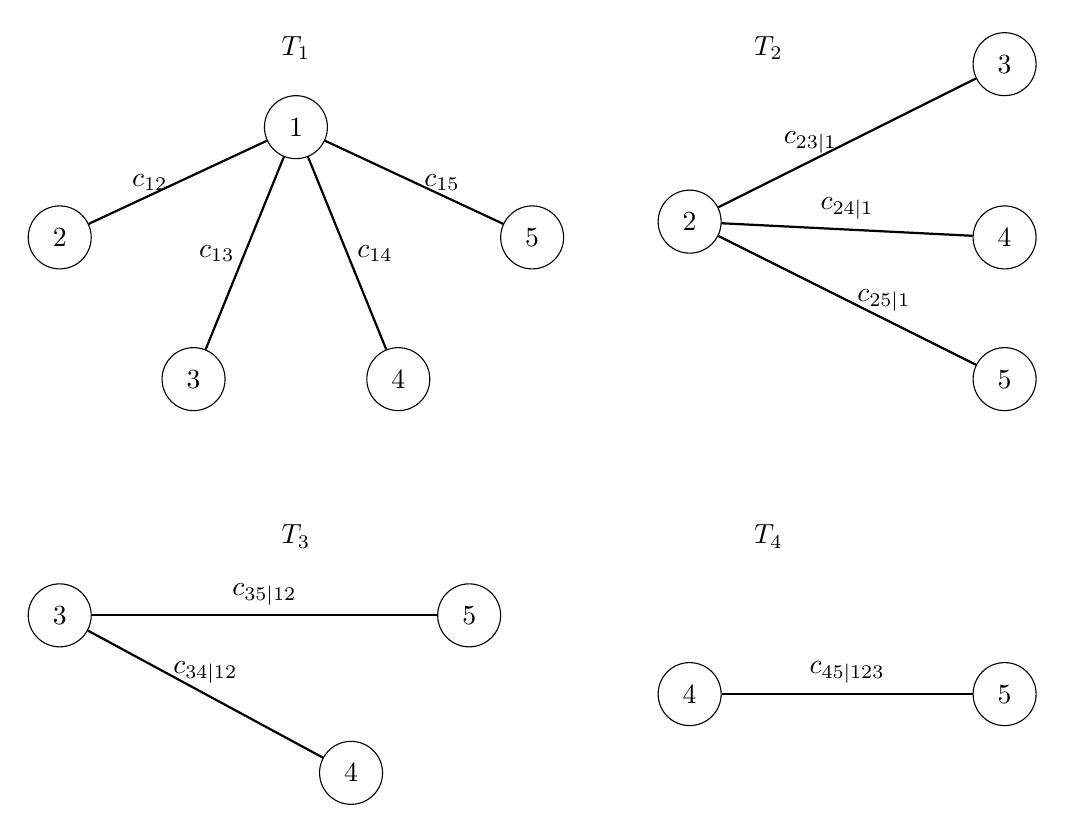
\begin{tikzpicture}[
						node/.style={
							circle,
							draw,
							minimum size=8mm,
							inner sep=0pt
						},
						edge/.style={thick}
						]

						% =========================
						% Tree 1
						% =========================
						\node at (0,3.2) {\textbf{$T_1$}};

						\node[node] (1) at (0,2.2) {$1$};
						\node[node] (2) at (-3,0.8) {$2$};
						\node[node] (3) at (-1.3,-1.0) {$3$};
						\node[node] (4) at (1.3,-1.0) {$4$};
						\node[node] (5) at (3,0.8) {$5$};

						\draw[edge] (1)--node[left]  {$c_{12}$} (2);
						\draw[edge] (1)--node[left]  {$c_{13}$} (3);
						\draw[edge] (1)--node[right] {$c_{14}$} (4);
						\draw[edge] (1)--node[right] {$c_{15}$} (5);


						% =========================
						% Tree 2
						% =========================
						\node at (6,3.2) {\textbf{$T_2$}};

						\node[node] (21) at (5,1) {$2$};
						\node[node] (22) at (9,3) {$3$};
						\node[node] (23) at (9,0.8) {$4$};
						\node[node] (24) at (9,-1) {$5$};

						\draw[edge] (21)--node[left]  {$c_{23|1}$} (22);
						\draw[edge] (21)--node[above] {$c_{24|1}$} (23);
						\draw[edge] (21)--node[right] {$c_{25|1}$} (24);


						% =========================
						% Tree 3
						% =========================
						\node at (0,-3) {\textbf{$T_3$}};

						\node[node] (31) at (-3,-4) {$3$};
						\node[node] (32) at (0.7,-6) {$4$};
						\node[node] (33) at (2.2,-4) {$5$};

						\draw[edge] (31)--node[above]  {$c_{34|12}$} (32);
						\draw[edge] (31)--node[above] {$c_{35|12}$} (33);


						% =========================
						% Tree 4
						% =========================
						\node at (6,-3) {\textbf{$T_4$}};

						\node[node] (41) at (5,-5) {$4$};
						\node[node] (42) at (9,-5) {$5$};

						\draw[edge] (41)--node[above] {$c_{45|123}$} (42);

					\end{tikzpicture}

					\caption{A cannonical vine with 5 variables, 4 trees and 10 edges.}
					\label{fig:c_vine_5d}
				\end{figure}


				\subsection{Akaike Information Criterion (AIC)}
				The AIC is an estimator of prediction error and relative quality of statistical models for given set of data. Given a collecion of models for the data, AIC estimates the quality of each model relative to each of the other models. And therefore, it can be used for model selection.
				\begin{thm}[\label{Thm:AIC}\cite{akaikeNewLookStatistical1974}]
					Let $M$ be a statistical model with $k$ estimated parameters. Let $\hat{L}$ be the maximised value of the log likelihood function for the model. Then , the AIC value of the model $M$ is
					\begin{equation} \label{Eq:AIC}
						AIC = 2k-2 \hat{L}.
					\end{equation}
				\end{thm}

				For a set of candidqte models, the preffered model is the one with the minimum AIC value.

				\textbf{Note:} from \ref{Eq:AIC}, AIC not only rewards goodness of fit but also penalises the increasing number of estimated parameters.


			\subsection{Basics of Bayesian Inference}
				\begin{defn}[Gamma function, $\Gamma$]
					For every positive integer $n$,
					\begin{equation}\label{eqn:gamma_int}
						\Gamma (n)=(n-1)!\,.
					\end{equation}
					For complex numbers with a positive real part, the gamma function is defined via a convergent improper integral:
						\begin{equation}\label{eqn:gamma_complex}
							\Gamma (z)=\int _{0}^{\infty }t^{z-1}e^{-t}{\text{ d}}t,\ \qquad \mathbb{R} (z)>0\,.
						\end{equation}
				\end{defn}

				\begin{defn}[Beta function, $\mathrm{B}$]
					It is defined by the integral

						\begin{equation} \label{eqn:beta}
							\mathrm {B} (z_{1},z_{2})=\int _{0}^{1}t^{z_{1}-1}(1-t)^{z_{2}-1}\,dt			\end{equation}
					for complex number inputs $z_{1},z_{2}$ such that $\mathbb{R}	 (z_{1}),\mathbb{R}(z_{2})>0$.
				\end{defn}
				A key property of the beta function is its close relationship to the gamma function:
				\begin{equation}
					\mathrm {B} (z_{1},z_{2})={\frac {\Gamma (z_{1})\,\Gamma (z_{2})}{\Gamma (z_{1}+z_{2})}}.
				\end{equation}
				\subsubsection{Beta distribution}
					The beta distribution is a family of continuous probability distributions defined on the interval $[0, 1]$ or $(0, 1)$ in terms of two positive parameters, denoted by $\alpha$ and $\beta$, that appear as exponents of the variable and its complement to 1, respectively, and control the shape of the distribution.
					In Bayesian inference, the beta distribution is the conjugate prior probability distribution for the Bernoulli, binomial, negative binomial, and geometric distributions. Its generalization to multiple variables is the Dirichlet distribution.

					\begin{defn}
						The probability density function (PDF) of the beta distribution, for $0 \le x \le 1$ or $0 < x < 1,$ and shape parameters $\alpha, \beta > 0,$ is a power function of the variable $x$ and of its reflection $(1 - x)$ as follows:
						\begin{equation}
							\begin{aligned}
								f(x; \alpha,\beta) &= constant \cdot x^{\alpha-1} (1-x)^{\beta - 1}\\
								&= \frac{x^{\alpha-1} (1-x)^{\beta - 1}}{\int_{0}^{1} u^{\alpha - 1}(1-u)^{\beta - 1} du}\\
								&= \frac{\Gamma (\alpha+\beta)}{\Gamma(\alpha)\Gamma(\beta)}x^{\alpha - 1}(1 - x)^{\beta - 1}\\
								&= \frac{1}{\beta(\alpha,\beta)}x^{\alpha - 1}(1 - x)^{\beta - 1}.
							\end{aligned}
						\end{equation}
					\end{defn}
				\subsubsection{Dirichlet distribution}
					The Dirichlet distribution often $Dir({\boldsymbol {\alpha }}),$ is a family of continuous multivariate probability distributions parameterized by a vector ${\boldsymbol {\alpha }}$ of positive reals.
					It is the continuous multivariate generalization of the Beta function and the conjugate prior of categorical and Multinomial distributions.
					The infinite-dimensional generalization of the Dirichlet distribution is the Dirichlet process.

				\begin{defn}[Dirichlet Distribution, \cite{Minka2012EstimatingAD}]
						The Dirichlet distribution of order $K \ge 2$ with parameters $\alpha_1, \dots, \alpha_K > 0$ has a probability density function with respect to Lebesgue measure on the Euclidean space $\mathbb{R}^{K-1}$ given by
						\begin{equation}
							f\left(x_{1},\ldots ,x_{K};\alpha _{1},\ldots ,\alpha _{K}\right)={\frac {1}{\mathrm {B} ({\boldsymbol {\alpha }})}}\prod _{i=1}^{K}x_{i}^{\alpha _{i}-1},
						\end{equation}
						where $\{x_{k}\}_{k=1}^{k=K}$ belong to the standard $K-1$ simplex, or in other words
						\begin{equation}
							\sum _{i=1}^{K}x_{i}=1{\mbox{ and }}x_{i}\in \left[0,1\right]{\mbox{ for all }}i\in \{1,\dots ,K\}.
						\end{equation}
						The normalizing constant is the multivariate beta function, which can be expressed in terms of the gamma function
						\begin{equation}
							\mathrm {B} ({\boldsymbol {\alpha }}) = {
								\frac {\prod \limits _{i=1}^{K}\Gamma (\alpha _{i})}
								{\Gamma \left(\sum \limits _{i=1}^{K}\alpha _{i}\right)}},
							\qquad {\boldsymbol {\alpha }}=(\alpha _{1},\ldots ,\alpha _{K}).
						\end{equation}
					\end{defn}
				\subsubsection{Multinomial distribution}
					The Multinomial distribution is a generalization of the binomial distribution. For example, it models the probability of counts for each side of a $k$-sided dice rolled $n$ times.
					The Bernoulli distribution models the outcome of a single Bernoulli trial. In other words, it models whether flipping a (possibly biased) coin one time will result in either a success (obtaining a head) or failure (obtaining a tail). The binomial distribution generalizes this to the number of heads from performing $n$ independent flips (Bernoulli trials) of the same coin. The Multinomial distribution models the outcome of $n$ experiments, where the outcome of each trial has a categorical distribution, such as rolling a $k-$sided die $n$ times.

					\begin{defn}[Multinomial distribution]
						Suppose one does an experiment of extracting $n$ balls of $k$ different colors from a bag, replacing the extracted balls after each draw. Balls of the same color are equivalent. Denote the variable which is the number of extracted balls of color $i (i = 1, ..., k)$ as $X_i$, and denote as $p_i$ the probability that a given extraction will be in color $i$. The probability mass function of this Multinomial distribution is
							\begin{equation}
									\begin{aligned}
										f(x_{1},\ldots ,x_{k};n,p_{1},\ldots ,p_{k})
											&= \Pr(X_{1}=x_{1}{\text{ and }}\dots {\text{ and }}X_{k}=x_{k})\\
											&={
												\begin{cases}{
														{n! \over x_{1}!\cdots x_{k}!} p_{1}^{x_{1}}\times \cdots \times p_{k}^{x_{k}}},\quad &{\text{when }}\sum _{i=1}^{k}x_{i}=n\\\\
														0	& {\text{otherwise,}}
												\end{cases}
											   }
									\end{aligned}
							\end{equation}
							for non-negative integers $x_1, \ldots, x_k$ \cite{berger2001statistical}.

							According to \cite{johnson1997multivariate}, the probability mass function can be expressed using the gamma function as
								\begin{equation}
									\begin{aligned}
										 f(x_{1},\dots ,x_{k};p_{1},\ldots ,p_{k})={\frac {\Gamma (\sum _{i}x_{i}+1)}{\prod _{i}\Gamma (x_{i}+1)}}\prod _{i=1}^{k}p_{i}^{x_{i}}.
									\end{aligned}
								\end{equation}
					\end{defn}

					This form shows its resemblance to the Dirichlet distribution, which is its conjugate prior.
				\subsubsection{Dirichlet - Multinomial distribution}
					The Dirichlet-Multinomial distribution is a compound distribution where a probability vector $p$ is drawn from a Dirichlet distribution with parameter vector $\alpha$ and then a sample of discrete outcomes $x$ is drawn from a Multinomial distribution with probability vector $p$ and number of trials $n$ \cite{Minka2012EstimatingAD}.
					\begin{defn}[Dirichlet - Multinomial Distribution]
						Given a random count vector $x=(x_1, \ldots, x_k)$ distributed according to a Multinomial distribution with a probability vector $p$ following a Dirichlet distribution with parameter vector $\alpha$. Then, following  \cite{Minka2012EstimatingAD}, the resulting distribution over $x$ a vector of outcomes is
						\begin{equation}
						 \begin{aligned}
						 	\Pr({x} \mid n,{\boldsymbol {\alpha }}) &=
								 	\int _{p }
									 	\mathrm {Mult} (x \mid n,p )
									 	\mathrm {Dir} (p \mid {\boldsymbol {\alpha }})dp\\
									 								&=
									 \int _{p }
									 	Pr(x \mid p)Pr(p \mid \boldsymbol{\alpha}) dp\\
									 								&=
									 {\frac {\Gamma \left(\alpha _{0}\right)\Gamma \left(n+1\right)}{\Gamma \left(n+\alpha _{0}\right)}}\prod _{k=1}^{K}{\frac {\Gamma (x_{k}+\alpha _{k})}{\Gamma (\alpha _{k})\Gamma \left(x_{k}+1\right)}}.
						 \end{aligned}
						\end{equation}
					\end{defn}

				\subsubsection{Bayes' Theorem}
				Let Pr(B,A) for the joint probability of events B and A.
				The relation between joint probabilities $Pr(B,A)$ and conditional probabilities $Pr(B|A)$ is the basis of Bayes’ theorem.
				\begin{defn}[Baye's Theorem]\label{dfn:bayestheorem}
					Consider the relation $ Pr(B,A) = Pr(B|A)Pr(A)$. If we switch the role of $A$ and $B$, we get $Pr(A,B) = Pr(A|B)Pr(B)$.

					Since $Pr(B,A)$ is the same as $Pr(A,B)$, we then have,
					\[
						Pr(B|A)Pr(A) = Pr(A|B)Pr(B).
					\]
					Hence
					\begin{equation}\label{eqn:baye_1}
						Pr(B|A) = \frac{Pr(A|B)Pr(B)}{Pr(A)}.
					\end{equation}
				\end{defn}


				Now suppose that instead of a single event $B$, we have a set $B_j,j = 1,2,. . . ,k$ of mutually exclusive and exhaustive events. The events $B_j$ being mutually exclusive and exhaustive, it follows that
				\begin{equation}\label{eqn:baye_2}
					Pr(A) = \sum_j Pr(A,B_j) = \sum_j Pr(A|B_j) Pr(B_j).
				\end{equation}

				\begin{thm}[Bayes' Theorem, \cite{link2009bayesian}]\label{thm:bayestheorem}
					Bayes’ theorem is established by substituting a specific event $B_i$ for $B$ in \eqref{eqn:baye_1}, and then substituting \eqref{eqn:baye_2} in the denominator of the right-hand side of \eqref{eqn:baye_1}. Thus Bayes’ theorem is that
					\begin{equation}
						Pr(B_i|A) = \frac{Pr(A|B_i)Pr(B_i)}{\sum_j Pr(A|B_j) Pr(B_j)}.
					\end{equation}
				\end{thm}

				The prior distribution $[\theta]$ (for parameter $\theta$) and the data distribution $[X|\theta]$ (for data $X$, given parameter $\theta$) are the core requirements for a Bayesian analysis. Bayes' theorem combines these according to theorem (\ref{thm:bayestheorem}) to produce the posterior distribution $[\theta|X]$ such that
				\begin{equation}\label{eqn:baye_3_1}
					[\theta|X] = \frac{[X|\theta][\theta]}{[X]},
				\end{equation}
				where
				\begin{equation}\label{eqn:baye_3_2}
					[X]=\int [X|\theta][\theta]d\theta.
				\end{equation}
				This posterior distribution summarizes all that is known about the parameter, combining prior knowledge and the information provided by the data and all the Bayesian inference is based on the posterior distribution. The data distribution, the prior, and the posterior, are the primary	features of Bayesian analysis. The distribution $[X]$ is the marginal distribution of the data. It is the average value of the data distribution, averaged against the prior. Since it need not be computed in characterizing the posterior distribution of $\theta$, equation \eqref{eqn:baye_3_1} may be written as
				\begin{equation}\label{eqn:baye_4}
					[\theta|X] \propto [X|\theta][\theta].
				\end{equation}
				Equation \eqref{eqn:baye_4} says that the posterior distribution is proportional to the product of the likelihood and the prior.

				Given data, $X$ and an unknown success rate, $p$, Bayesian analysis of the data $[X]$ requires nothing more than specification of a prior distribution $[p]$. There is great flexibility in the choice of prior: $[p]$ can be any distribution on $[0, 1]$ and  Bayesian inference includes a formal mechanism for updating prior knowledge. If one chooses a prior which expresses dead certainty about the value of the parameter, then the data will be ignored; however, if the prior expresses uncertainty about the parameter, then as sample size increases, the data will prevail in guiding inference.

				\subsection{How to Choose a Good Prior}
				There are two considerations to note:
				\begin{enumerate}
					\item[(i.)] Certain families of prior distributions are very naturally chosen, on the grounds of convenience and expositional clarity. For example a beta distribution as prior for the binomial distribution success parameter. Here, the beta family of distributions is said to be \textit{conjugate} for the binomial success parameter i.e the prior and the posterior distributions are in the same family. The beauty of this is 		that the posterior from one study is ready made to serve as prior in the next.\\
					There is also a computational efficiency associated with using a conjugate prior: the posterior being of known form, there is no need to compute the integral in equation \eqref{eqn:baye_3_2}.

					\item[(ii.)] Analysts often wish to let the data speak for itself, as much as possible.
				\end{enumerate}

				When an objective Bayesian analysis is desired for the binomial success rate $p$, a common choice of prior is the uniform distribution on $[0, 1]$. A uniform prior on $p$ says that we have no more reason to believe it falls in any particular sub-interval of $[0, 1]$ than in any other of the same length\cite{link2009bayesian}.

			\subsubsection{Calculating Posterior Distributions}
				In equation \eqref{eqn:baye_3_1}, the only role of the denominator $[X]$ in defining the posterior is as a “normalizing constant,” a scaling factor included so that the posterior distribution integrates to 1. Thus, it is simply written as Equation \eqref{eqn:baye_4}. While we do not need $[X]$ to define the posterior, we do need it if we are to calculate features such as its mean, variance, its percentiles; we may want to specific probabilities such as $Pr(\theta >0|X)$.

				$[X]$ is found by averaging the data distribution $[X|\theta]$ against the prior $[\theta]$ as in equation \eqref{eqn:baye_3_2}. However, evaluating this integral is almost always difficult and frequently impossible. Here, we describe a variety of methods for getting around this difficulty, so that we may evaluate posterior distributions.

			\subsubsection{Conjugacy}
				Identifying posterior distributions is easy when we can identify a family of distributions, which includes both the prior and posterior distributions. Distributions in this "conjugate family" are identified by a hyper-parameter $\Lambda$.
				What is known before data collection is summarized by a particular value $\Lambda_0$ and what is known afterwards by a new value $\Lambda_1$. The process of updating knowledge by data boils down to updating $\Lambda$, and the transition from $\Lambda_0$ to $\Lambda_1$ involves simple summaries of the data.

				\textbf{Note:} The existence of a conjugate family depends on the form of the likelihood function.

				\subsubsection{Binomial likelihood:}
					Consider events modeled as Bernoulli trials. If the trials are independent, the data distribution $Y$ is binomial, $Y \sim B(N,p)$ with $p$ denoting the unknown probability.

					Suppose that our prior knowledge about $p$ can be represented by a beta distribution with parameters $a_0$ and $b_0$. Then,
					\begin{equation*}
						\begin{aligned}
							[p|Y] &\propto [Y|p]\times[p]\\
							&\propto p^{Y}(1-p)^{N-Y} \times p^{a_0}(1-p)^{b_0-1}\\
							&=p^{a_1-1}(1-p)^{b_1-1}
						\end{aligned}
					\end{equation*}
					where $a_1 = Y+a_0$ and $b_1 = N-Y+b_0$.

					Since the posterior distribution must integrate to 1, it must actually be a beta distribution; thus,
					\[
						[p|Y] = \frac{\Gamma(a_0+b_0+N)}{\Gamma(a_0+Y)\Gamma(b_0+N-Y)}p^{a_0+Y-1}(1-p)^{b_0+N-Y-1}.
					\]

					Given the binomial likelihood, and a beta prior, we obtain a beta posterior: \textit{the beta family of priors is conjugate for the binomial likelihood.} The hyper-parameter $\psi = \{ a,b\}$ is updated by adding the number of successes to $a_0$, and the number of failures to $b_0$.
					In the absence of specific knowledge, the choice $a_0 = 1$ and $b_0 = 1$ may be reasonable, since it describes a uniform prior on $p$ \cite{link2009bayesian}.

				\subsubsection{Poisson Likelihood:}
					Let $Y = { y_1,. . . ,y_n}$ denote the observed values in a random sample drawn from a Poisson distribution with parameter $\lambda$, and suppose that the prior for $\lambda$ is a gamma distribution with parameters $\alpha_0$ and $\beta_0$. We find that the posterior distribution $[\lambda|Y ]$ is given by
					\begin{equation*}
						\begin{aligned}
							[\lambda|Y] &\propto \prod_{i=1}^{n}\frac{e^{-\lambda}\lambda^{y_i}}{y_i!} \times \frac{\beta^{\alpha_0}_0}{\Gamma(\alpha_0)}\lambda^{\alpha_0 -1}e^{-\beta_0\lambda}\\
							&\propto (e^{-n\lambda}\lambda^{n\bar{y}})\times (\lambda^{\alpha_0-1}e^{-\beta_0\lambda})\\
							&=\lambda^{\alpha_1-1}e^{-\beta_1\lambda},
						\end{aligned}
					\end{equation*}
					where $\alpha_1 = n\bar{y}+\alpha_0$ and $\beta_1=n+\beta_0$.
					Thus the posterior distribution is in the same family as the prior; both are gamma distributions. \textit{The gamma family of priors is conjugate for the Poisson likelihood.} The hyper-parameter $\psi = \{ \alpha,\beta \}$	is updated by adding the total count to $\alpha_0$, and the sample size to $\beta_0$ \cite{link2009bayesian}.


				\subsubsection{ Multivariate Posterior Distribution:}
					With more than one unknown, inference is based on a multivariate (joint) posterior distribution. This distribution is of the same form as Eq. \eqref{eqn:baye_3_1}, but now the parameter $\theta$ is vector valued, and $[\theta|X]$ is a multivariate distribution. More often, inference focuses on one parameter at a time.

					For a vector-valued parameter $\theta = (\theta_1,\theta_2,\dots,\theta_k)'$, Eq. \eqref{eqn:baye_4} becomes \[[\theta|X] \propto [X|\theta][\theta],\] that is, \[ [\theta_1,\dots,\theta_k|X] \propto [X|\theta_1,\dots,\theta_k][\theta_1,\dots,\theta_k]. \]

					To make inference about a single parameter, we examine the marginal posterior for the parameter of interest. For example, the marginal posterior distribution for parameter $\theta_1$ is found by, \[ [\theta_1|X] = \int\dots\int [\theta_1,\dots,\theta_k|X]d\theta_2,\dots, \theta_k. \]

					So inference for a single parameter in a multi-parameter setting involves two potentially difficult calculations: first, of the joint posterior, second, of the marginal posterior from the joint.

					There are cases where conjugate priors exist for multivariate parameters. This makes the first task, of identifying the joint posterior, feasible. Otherwise, the two tasks are easily accomplished by the simulation techniques \cite{link2009bayesian}.


			\subsection{Monte Carlo Methods:}
				The basic idea of simulations is that we can study features of a probability distribution $F$ 	by examining corresponding features of a sample $X_1, X_2, . . . , X_n$ from $F$.

				\subsubsection{Cdf Inversion:}
					This is the easiest method for scalar (uni-variate) random variables.
					Suppose that $X$ is a continuous random variable with cumulative distribution function (cdf ) $F(t) = Pr(X \le t)$.
					$F(t)$ is monotone increasing, hence invertible, that is, there exists a function $F^{-1}$ such that $F^{-1}(F(t)) = F(F-1(t)) = t$.
					Since $Pr(X \le t) = F(t), Pr(F(X) \le t) = Pr(X \le F^{-1}(t)) = F(F^{-1}(t)) = t$, for all $t\in [0, 1]$. So $F(X)$ has the same distribution as a uniform random variable $U \sim U(0,1)$, from which it follows that $F^{-1}(U)$ has the same distribution as $X$.

				\subsubsection{Rejection Sampling:}
					Rejection sampling is a simple technique for changing a sample from a distribution $c(x)$ into a (smaller) sample from another distribution $t(x)$. It is useful when it is easy to sample from the candidate distribution, $c(x)$ but difficult to directly sample the target distribution, $t(x)$.

					\textbf{Proceedure:}
					\begin{enumerate}
						\item[i.] Choose an easily sampled candidate distribution $c(x)$, ensuring that there is a number $M < \infty$ such that over the entire range of $t(x), t(x) \le Mc(x)$.
						\item[ii.] Draw a sample $X ~ c(x)$ and calculate $w(X) = t(X)/(Mc(X))$. Note that $0 \le w(X) \le 1$.
						\item[iii.] We conduct a Bernoulli trial with success probability $w(X)$; if the trial is successful, the value
						$X$ is accepted as an observation from $t(x)$, otherwise, the value is discarded.
					\end{enumerate}

			\subsection{Markov Chain Monte Carlo (MCMC):}
				This is a simulation technique for examining probability distributions.

				\subsubsection{Metropolis-Hastings Algorithm:}
					\textbf{Proceedure:}
					Suppose that we wish to draw samples from target distribution $f(x)$.  Let $j(x|y)$ be candidate generating distributions, describing probabilities for candidate values $x$, given current value $y$.
					Fix a value $X_0$. Then for $t=1,2,\dots$, generate $X_t$ according to the following rules:
					\begin{enumerate}
						\item Generate a candidate value, $X_{cand}$ by sampling from $j(x|X_{t-1}).$
						\item Calculate $$r =\frac{f(X_{cand})j(X_{t-1}|X_{cand})}{f(X_{t-1})j(X_{cand}|X_{t-1})}.$$
						\item Generate $U \sim U(0,1).$
						\item If $U<r$, set $X_t = X_{can.d}$, otherwise set $X_t = X_{t-1}.$
					\end{enumerate}

					Notice that in the algorithm, the target distribution is only involved in calculating $r$, and it occurs in both the numerator and the denominator. Hence if $f$ is a posterior distribution equation \eqref{eqn:baye_3_2} ($[X]$), the normalizing constant cancels out.

				\subsubsection{Gibbs Sampling:}
					This is designed for multi-variate posterior distributions. Given $\theta=(\theta_1,\theta-2,\dots,\theta_k)'$ represent unknown quantities, and $X$ represent data. the goal then is to draw a sample from $[\theta|X]$

					\textbf{Algorithm:}
					Suppose that we wish to draw samples from a joint posterior distribution $[\theta|X]$.\\
					Fix a value $\theta^{(0)} = (\theta^{(0)}_1 ,\theta^{(0)}_2,\dots ,\theta^{(0)}_k)'$. Then for $t= 1,2,\dots$, generate $\theta^{(t)}$ according to the following rules:
					\begin{enumerate}
						\item Sample $\theta_1^{(t)}$ from
						\[
						[\theta_1 \mid \theta_2^{(t-1)},\ldots,\theta_k^{(t-1)},X].
						\]

						\item For $j=2,\ldots,k$, sample $\theta_j^{(t)}$ from
						\[
						[\theta_j \mid
						\theta_1^{(t)},\ldots,\theta_{j-1}^{(t)},
						\theta_{j+1}^{(t-1)},\ldots,\theta_k^{(t-1)},X].
						\]

						\item Set
						\[
						\theta^{(t)}
						=
						\left(
						\theta_1^{(t)},\theta_2^{(t)},\ldots,\theta_k^{(t)}
						\right)'.
						\]
					\end{enumerate}

					%\begin{enumerate}
					%	\item Sample $\theta_1^{(t)}$ from the full conditional $[\theta_1|\theta^{(t-1)}_{(-1)},X]$.
					%	\item Sample $\theta_2^{(t)}$ from the full conditional $[\theta_2|\theta^{(t-1)}_{(-2)},X]$.
					%\end{enumerate}
					%\dots
					%\begin{enumerate}
					%	\item Sample $\theta_k^{(t)}$ from the full conditional $[\theta_k|\theta^{(t-1)}_{(-k)},X]$.
					%\end{enumerate}
					%\begin{enumerate}
					%	\item Set  $\theta^{(t)} = (\theta^{(t)}_1 ,\theta^{(t)}_2,\dots ,\theta^{(t)}_k)'$.
					%\end{enumerate}

					\textbf{Note:} It is also acceptable to sequentially update $\theta^{(t)}$ after each step in the preceding algorithm, and to use the partially updated $\theta^{(t)}$ in sampling subsequent full conditionals. For instance, $\theta^{(t)}_3$ could be sampled from the full conditional distribution
					\[
						[\theta_3|\theta_1^{(t)},\theta_2^{(t)},\theta_4^{(t-1)},\dots,\theta_k^{(t-1)},X],
					\]rather than
					\[
						[\theta_3|\theta_1^{(t-1)},\theta_2^{(t-1)},\theta_4^{(t-1)},\dots,\theta_k^{(t-1)},X].
					\]


			\subsection{Mean-Variance Efficiency}
				Consider $P$ assets with random returns $\tilde{\xi} = (\tilde{\xi}_1,\dots,\tilde{\xi}_P)$. Let $w=(w_1,\dots,w_P)$ be the proportion variables and these weights are constrained via $w\in \mathbb{W}= \{w:\sum_{i=1}^{P}w_i=1,w\ge 0\}$.
				Let $\tilde{R}_w = w^T\tilde{\xi}$ be the random return of the manager's portfolio and $R_w$ and $\xi$ be the realizations of $\tilde{R}_w$ and $\tilde{\xi}$ respectively.
				The manager's goal is to find an allocation $w^*$ which solves
				\begin{equation}\label{Eq:obj1}
					w^* = \max_{w\in\mathbb{W}	} Eu(\tilde{R}_w),
				\end{equation}
				where $u$ is a real-valued utility function that represents the manager's objectives.

				We assume $Eu(\tilde{R}_w)$ is upper semi-continuous on $\mathbb{W}$ and since $\mathbb{W}$ is compact, it ensures that \eqref{Eq:obj1} has a finite optimal solution, $w^*$, which is achieved on $\mathbb{W}$.

				For maximizing the probability that the benchmark is achieved, consider $u$ to be a utility function that depends on a benchmark return $R_b$ which can be random or deterministic.
				\begin{equation}\label{Eq:utilfunc}
					u(R_w) = I(R_w \ge R_b),
				\end{equation}
				where $I(\cdot)$ takes 1 if the argument is true and 0 otherwise.
				\begin{defn}\label{dfn:mean-var}
					The mean efficient frontier can be defined as
					\begin{equation*}\label{Eq:mean-eff}
						\resizebox{\hsize}{!}{
							$\mathcal{F} = \{
							(\mu,\sigma^2) :
							\exists w\in \mathbb{W} \text{ with }  \mu_w=\mu, \sigma_w^2=\sigma^2 \text{ and }
							\not\exists \hat{w}\in \mathbb{W} \text{ with }  \mu_{\hat{w}} \ge \mu, \sigma_{\hat{w}}^2 < \sigma^2
							\}
							$}
					\end{equation*} where $\mu_w = \sum_{i=1}^{p}E\tilde{\xi}_i w_i$ and $\sigma_w^2 = \sum_{i=1}^{p}\sum_{j=1}^{p} cov(\tilde{\xi}_i \tilde{\xi}_j)w_i w_j$.
					A feasible allocation decision $w\in\mathbb{W}$ is said to be on efficient frontier if $(\mu_w,\sigma-w^2) \in \mathcal{F}$.
				\end{defn}

				\begin{lem}[\cite{morton2003optimizing}]\label{lem:mean-eff}
					Assume $Eu(R_w)$ can be expressed as $Eu(R_w) = F(\mu_w,\sigma_w^2)$ for some function $F$ and let $w^*$ solve equation \eqref{Eq:obj1}. If $ F(\mu_w,\sigma_w^2)$ is increasing in $\mu_w$ and decreasing $\sigma_w^2$, then $w*$ is on the efficient frontier.
				\end{lem}
				Assuming $\xi$ has a multivariate normal distribution, $\Phi$ is the CDF of a standard normal, and let $m_w = R_b-\mu_w$. If the benchmark is random, then $\tilde{\xi}  \leftarrow \tilde{\xi}-R_b$ and use a deterministic benchmark of 0. In this case, $m_w = -\mu_w$.

				Under the multivariate normal hypothesis,
				\begin{equation}\label{Eq:Phi}
					P(\tilde{R}_w \ge R_b) = 1 - \Phi(\frac{m_w}{\sigma_w}).
				\end{equation}
				Note that in our problem, the benchmark is random and so $R_b = 0$. Hence
				\begin{equation}
					P(\tilde{R}_w \ge R_b) = 1 - \Phi(\frac{-\mu_w}{\sigma_w}).
				\end{equation}
				Equation \eqref{Eq:Phi} establish the existence of an $F(\mu_w,\sigma_w^2)$ function for the expected utility function which allows us to explore conditions under which the monotonicity hypothesis of $F$ in lemma 1 are satisfied.

				\begin{thm}[\cite{morton2003optimizing}]\label{thm:argmax_on_eff}
					Let $\tilde{\xi}$ be multivariate normal. If there exists $\hat{w} \in \mathbb{W}$ with $\mu_{\hat{w}} > R_b$, then $w^* \in  \argmax_{w \in \mathbb{W}} Eu(\tilde{R}_w)$ is on the efficient frontier.
				\end{thm}

				Theorem \ref{thm:argmax_on_eff} says that when maximizing the probability of achieving the benchmark, mean-variance efficiency is obtained if we also assume there exists $\hat{w} \in \mathbb{W} \text{ with } \mu_{\hat{w}} > R_b$ such that

				\begin{equation}\label{Eq:maxProb2}
					\max_{w\in\mathbb{W}}Prob(R_w-R_b \ge 0)
				\end{equation}



			\subsection{Solution procedures and the solution quality} \label{sec:sol_to_mean_var}
				\begin{propn}[\cite{morton2003optimizing}]

					Assume that the returns are normally distributed i.e. $R_w-R_b \sim N(\mu_w,\sigma_w^2)$. Consider that $Eu(\tilde{R}-w)$ is not concave or its concavity has not been established. If we assume that mean-variance efficiency has been established, we know that the solution is in the set
					\begin{equation}\label{Eq:muge}
						\{ w(\lambda):w(\lambda) \in \argmax_{w\in \mathbb{W}} \mu_w - \lambda\sigma_w^2, \lambda \ge0 \}.
					\end{equation}

					If $\mu_w <0$ for all $w\in \mathbb{W}$, then,
					\begin{equation}\label{Eq:mule}
						\{ w(\lambda):w(\lambda) \in \argmax_{w\in \mathbb{W}} \mu_w + \lambda\sigma_w^2, \lambda \ge0 \}.
					\end{equation}
				\end{propn}

				Equations \eqref{Eq:muge} and \eqref{Eq:mule} can be generated via parametric quadratic binary programming. And according to \cite{morton2003optimizing}, this reduces the $p$-dimensional optimal allocation problem to a line search about $\lambda$. In other wards, we choose the value of $\lambda$ that yields the largest objective in \eqref{Eq:maxProb} or \eqref{Eq:Phi}. According to \cite{sun2006optimization}, we can find the solution to the line search using the Forward-Backward Method.



		\chapter{Literature Review}
			Fantasy games can be traced back to Wilfred ‘Bill’ Winkenbach. He created fantasy golf and football rules in the late 1950s and early 1960s. In 1984, Charpentier and Tom Kane Jr. Co-authored "The Fantasy Football Digest '', explaining fantasy football rules. The game was later popularized, first through magazines and then through newspapers.  Back then, putting together a lineup and getting results was an uphill task accomplished by posting through the mail. With the arrival of the internet, information and online fantasy games became readily available to fantasy managers worldwide, simplifying the process of managing fantasy teams. Since then, interest in fantasy sports has grown to include 62.5 million players in the USA and Canada\cite{IndustryResearch}, 160 million in India, and 9.1 million globally in the Fantasy Premier League (FPL) by 2022\cite{HowManyPeople2022}.

			With such popularity and its disposition as an interesting intellectual challenge, it wasn’t long before the mathematicians came knocking. Much work has since been published on fantasy games from various perspectives. For example, \cite{Kaplan_Garstka_2001}  and \cite{Clair_Letscher_2007} modeled tournaments to predict the maximum number of game winners in an upcoming elimination tournament. Regarding head-to-head contests, \cite{becker2016analytical} attempted the first analytical approach to line-up management in the context of an entire NFL season, i.e., encompassing the draft, weekly play, and playoff phases. They develop a mixed integer programming model that caters to all phases but is biased towards the draft phase. They also modeled opponents' behaviors based on expert player rankings before the draft, i.e., when it is their turn, the opponent is expected to draft the most highly ranked remaining player to their team. However, this game format diverges significantly from the FPL Head-to-Head game in many aspects: Firstly, it is structured so that each player belongs to only one team in the competition; Secondly, you keep the same team for the entire season. Therefore, we cannot directly apply the tools developed in this work to H2H in FPL.

			More closely related to our problem is the work by \cite{haugh2021play} who devised a framework for assembling daily fantasy teams to compete in pool-style competitions. In these competitions, a manager typically competes against thousands of opponents for a monetary cash prize. For each round of games, managers can freely select any player into their team despite their opponents’ choices. They model opponents’ choices using Dirichlet regression and use these to determine the stochastic benchmark to beat for a win. This approach is well suited for the H2H competition in FPL since we know our opponents in advance and can extract information about their player selection patterns from their previous match-ups. The probability of outperforming the stochastic benchmark is optimized by subjecting it to game constraints. A H2H match-up in FPL can be considered a special case of pool-style competitions with only two players. However, adjustments were made before Haugh et al. \cite{haugh2021play}’s was utilized framework for our problem. These include accommodations for
			\begin{enumerate}
				\item[-] A more extended planning period due to restrictions on changing the team in future game weeks. We intend to optimize for 2-3 game weeks using ideas from  \cite{becker2016analytical}.
				\item[-] A single opponent to beat. The pool size was expanded by considering all combinations generated by possible transfers and substitutions from the bench.
				\item[-] Free-hits and wildcard chips where a manager is allowed to freely overhaul their team. This is particularly important when modeling the opponent’s team, as this could significantly undermine our chances of winning that match-up.
			\end{enumerate}

		\chapter{Problem Formulation and Results} \label{chap:formulation}
			\section{Mathematical formulation for the Problem}
			Using a similar procedure as \cite{haugh2021play}, our goal is to choose a squad   $\omega \in \{0,1\}^P$.

				\subsection{Assumptions:}
					\begin{itemize}
						\item There is a total of $P$ real-world players whose performance   $\delta \in Z^P$in a given game week is random.
						\item $\delta$ has mean vector $\mu_{\delta}$ and variance-covariance matrix $\Sigma_{\delta}$.
						\item Projected Player performance will determine the available player pool from which we make transfers.
					\end{itemize}

				\subsection{Feasibility constraints}
					Typically, there are many constraints on $\omega$ . For example, in a typical FPL contest,
					\begin{itemize}
						\item We are only allowed to select $C = 15$ athletes out of $P$ FPL players, each athlete having a certain cost and the team would not exceed a given budget $B=100$ million fantasy dollars.

						These constraints on $w$ were formulated as follows
						\[
						\begin{aligned}
							\sum_{i=1}^{P}\omega_i &=C,\\
							\sum_{i=1}^{P}c_i\omega_{i} &\le B,
						\end{aligned}
						\]
						where $\omega_{i} \in \{0,1\}, i = 1, ..., P$, and $c_i$ is the cost the $i^{th}$ athlete.
						\item There are also positional constraints on $\omega$ such as for each squad that is selected, we should have 2 goalkeepers, $g$ , 5 defenders, $d$ , 5 midfielders, $m$ , and 3 forwards $f$. This has the following formulation;
						\[
						\begin{aligned}
							\sum_{i=1}^{P_g}\omega_{i} =g\\
							\sum_{i=1}^{P_d}\omega_{i} =d\\
							\sum_{i=1}^{P_m}\omega_{i} =m\\
							\sum_{i=1}^{P_f}\omega_{i} =f,
						\end{aligned}
						\]
						where $\omega \in \{0,1\}$, and $P_g+P_d+P_m+P_f=P$.
						\item Any combination of $c_{in}=11$ Players (line-up) from the different positions can be formed from the squad of 15 players given that the combination includes 1 goalkeeper, at least 3 defenders, at least 2 midfielders, and at least 1 forward. These are formulated as below;
						\begin{itemize}
							\item The 11 player squad is given by $\sum_{i=1}^{P}\sum_{j=1}^{C}\omega_{i,j} = c_{in}$ where $\omega_{i,j}$ is the $j^{th}$ player in $\omega_{i}$.

							Also, $\sum_{i=1}^{P}\sum_{j=1}^{C_g}\omega_{i,j} = 1, \sum_{i=1}^{P}\sum_{j=1}^{C_d}\omega_{i,j} \ge 3, \sum_{i=1}^{P}\sum_{j=1}^{C_m}\omega_{i,j} \ge 2, \sum_{i=1}^{P}\sum_{j=1}^{C_f}\omega_{i,j} \ge 1$, where $C_g+C_d+C_m+C_f = C$.
						\end{itemize}

					\end{itemize}

				\subsection{The Problem}

					Let $\mathbb{W}$ be the set of binary tuples $\omega \in  \{0,1\}$ that satisfy the above constraints.

					Following Haugh. et. al.\cite{haugh2021play}, we assumed that for each a particular opponent, there are $O$  possible squad combinations that they could field in upcoming game week and let $\mathbb{W}_o = \{\omega_i\}^O_{i=1}$ denote these possible squad combinations the opponent could field in the upcoming game week.
					We assume that making changes to $c_{in}=11$ player squad from the $C=15$ will result in a new $\omega_i$. $\mathbb{W}_{o}$ will be computed as a combination of the following;

					\begin{enumerate}
						\item[i.] Opponent’s current 15 player squad will result in 550 squad combinations as shown below:
						\begin{itemize}
							\item 	Given that each combination of 11 players  $c_{in}=11$ should have 1 goalkeeper, at least 3 defenders, at least 2 midfielders and at least 1 forward, we can then have the following combinations;
							\begin{table}[ht]
								\begin{center}
									\begin{tabular}{|l|l|}
										\hline
										Allowed Formations (GK, DEF, MID, FWD)& Combinations\\
										\hline
										1-3-4-3 & $C_1^2 \cdot C_3^5 \cdot C_4^5 \cdot C_3^3 =30$\\
										\hline
										1-3-5-2 & $C_1^2 \cdot C_3^5 \cdot C_5^5 \cdot C_2^3=60$\\
										\hline
										1-4-3-3 & $C_1^2 \cdot C_4^5 \cdot C_3^5 \cdot C_3^3=100$\\
										\hline
										1-4-4-2 & $C_1^2 \cdot C_4^5 \cdot C_4^5 \cdot C_2^3=150$\\
										\hline
										1-4-5-1 & $C_1^2 \cdot C_4^5 \cdot C_5^5 \cdot C_1^3=30$\\
										\hline
										1-5-2-3 & $C_1^2 \cdot C_5^5 \cdot C_2^5 \cdot C_3^3=20$\\
										\hline
										1-5-3-2 & $C_1^2 \cdot C_5^5 \cdot C_3^5 \cdot C_2^3=60$\\
										\hline
										1-5-4-1 & $C_1^2 \cdot C_5^5 \cdot C_4^5 \cdot C_1^3=30$\\
										\hline
										Total   & 550\\
										\hline
									\end{tabular}
								\end{center}
								\caption{A table showing the squad combinations for an opponent}
							\end{table}

						\end{itemize}
						\item[ii.] If 1 playing transfer is made, the we have more $550 \cdot [C_1^{n_g} +C_1^{n_d}+C_1^{n_m} +C_1^{n_f}]$.
						\item[iii.] If 2 playing transfer is made, the we have more $550 \cdot  [C_2^{n_g} +C_2^{n_d}+C_2^{n_m} +C_2^{n_f}]$.
					\end{enumerate}

					Hence
					\begin{equation*}
						\begin{aligned}
							O &= 550 \cdot (1 + [C_1^{n_g} +C_1^{n_d}+C_1^{n_m} +C_1^{n_f}] + [C_2^{n_g} +C_2^{n_d}+C_2^{n_m} +C_2^{n_f}])\\
							&= 550 \cdot  (1 + C_1^{n_g} +C_1^{n_d}+C_1^{n_m} +C_1^{n_f} + C_2^{n_g} +C_2^{n_d}+C_2^{n_m} +C_2^{n_f}),
						\end{aligned}
					\end{equation*}
					where $n_g,n_d,n_m$, and $n_f$ is the number/pool of available goalkeepers, defenders, midfielders and forwards respectively, from which we can make transfers.

					At the end of the game week, our squad, $\omega$ , realizes a points total of $F=\omega^T\sigma$ and our opponent’s possible realized points totals are $G_i=\omega_i^T\delta$  for $i = 1,\dots,O$. All squads $\omega_o$’s are then ranked according to their points total in $\{G_i\}^O_{i=1}$.

					Using the double-up from formulation from Haugh et. al\cite{haugh2021play}, we would like $\mathbb{W}$ to be in the top $r$ teams with $N=1$ and $r =\frac{(O+1)}{k}$ for $0 < k<O$ and $k$ is the factor by which the payoff is multiplied by. For a double-up $k=2$, for a quintupple, $K=5$, and so on.
					The fantasy team optimization problem then is to solve,
					\[
					\max_{\omega \in \mathbb{W}} Prob\{\omega^T\delta > G^{(r')}(\mathbb{W}_o,\delta)\},
					\]
					where $G^{(r)}$ is the $r^{th}$ order statistic of $\{G_i\}_{i=1}^O$ and $r' =O+1-r$.
					$r$ is 50\% for a risk-neutral manager who just wants to beat 50\% of the opponent's possible teams but could rise as high as 90\% for a risky manager.

%			\section{Methodology}
%				The following methods shall be employed to achieve the stated specific objectives:
%				\subsection{Specific objective 1}
%				We used clear and universal mathematical notation for problem formulation, apply mathematical analysis techniques to understand solution characteristics and borrow any pertinent results from mathematical finance. This approach ensured a rigorous and quantitatively sound framework that balances theoretical accuracy with practical relevance in decision-making.
%
%				\subsection{Specific objective 2}
%				We used data from diverse sources such as the FPL API, Github, Understat.com, and web scraping of online bookmakers to develop machine learning models. This comprehensive dataset contains both historical data and information on future game conditions, such as fixture difficulty ratings. It enabled us to develop robust predictions for player performances in upcoming game weeks.

%				\subsection{Specific objective 3}
%				We collected information on current player ownership and transfer trends and analyze historical data on opponent team selections and captain choices. This data informed the Dirichlet-multinomial model, which allowed us to incorporate prior knowledge and update our predictions based on the new information. This offered a dynamic and statistically robust method for anticipating opponents' strategies. Marginal distributions for each player were then be used for selection. Key ingredients to the selection parameters were be the predicted performance and extra cost of bringing in a new player.
%				\subsection{Specific objective 4}
%				Based on the above predictions for player performance and opposition line-up, we utilized efficient optimization techniques to recommend the best selections and transfers for the current game week with considerations for the upcoming game week(s).

%				\subsection{Specific objective 5}
%				We used suitable statistical tests to determine if the differences in performance between our framework and conventional methods are significant.

		\section{Modeling Opponents' team selection}
			Each team has $C=15$ positions which must consist of 2 goalkeepers, ($g$), 5 defenders ($d$), 5 midfielders($m$), and 3 forwards ($f$).

			Let $w_o = (w^g,w^d,w^m,w^f)$; $w^g$ denotes the goalkeeper component of $w_o$, $w^d$ denotes the defender component of $w_o$, etc and we refer to them as the positional marginals of $w_o$. If there are $P_g$ goalkeepers available for selection, then $w_o^g \in \{0,1\}^{P_g}$ and exactly 2 components of $w_o^g$ will be 1 for any feasible $w_o$.Hence $P_g+P_d+P_m+P_f=P$ since there $P$ athletes in total available for selection.

			Using Sklar's theorem \ref{thm:sklar}, we can model the distribution of $w_o$. We can then write;
			\begin{equation}\label{Eq:sklarapp}
				F_{w_o}(w^g_o,w^d_o,w^m_o,w^f_o) = C(F_g(w^g_o),F_d(w^d_o),F_m(w^m_o),F_f(w^f_o)),
			\end{equation}
			where $F_{w_o}$ denotes the CDF of $w_o$, $F_g, F_d, F_m, \text{ and }F_f$ represent the margin CDFs of $w_o^g, w_o^d, w_o^m, \text{ and } w_o^f$ respectively, and $C$ is the copula of $w_o^g,w_o^d,w_o^m,w_o^f$.
			$C$ which is only defined on $Range(F_g)\times \dots \times Range(F_d)$ models the dependence structure of the positional marginals.

			Using Sklar's theorem in (\ref{Eq:sklarapp}), in order to determine the distribution of $w_o$ , we now only need to deal with 2 separate sub-problems;
				\begin{enumerate}
					\item[(i).] Modeling and estimating the positional marginals $F_g, F_d, F_m, \text{ and }F_f.$
					\item[(ii).] Modeling and estimating the copula of $w_o^g,w_o^d,w_o^m,w_o^f$.
				\end{enumerate}

			\subsection{Estimating positional margins}
				Modelling the positional margins for the opponent means we are tracking the opponent's squad transisition through the gameweeks. To do this, we employ a two-stage Bayesian Hierachical modelling.
				First, we estimate the cross-sectioanl parameters for the league. These parameters then serve the league baseline or priors for the longitudinal parameter estimtion for the opponent's team selection modelling.

				\subsubsection{The Cross-sectional League Baseline (Prior)}
				Here, we pool the team seelction data for all the league managers for a specific gameweek $t$. Let $j \in \{g,d,m,f\}$ be the positions in the squad, $N_j$ be the number of players in position $j$, and $p_j = \{p_j^k\}_{k=1}^{P_j}$ lie on the simplex in $\mathbb{R}^{P_j}$.

				If $p_{j,t} \sim Dir(\alpha^{league}_{j,t})$, where $Dir (\alpha^{league}_j)$ denotes the Dirichlet distribution with parameter vector $\alpha^{league}_j$ and a random opponent selects a player $k_j$ with probability $p_j^{k_j}$ for $k_j = 1, ..., P_j$. The chosen player follows a $Multinomial(N_j, p_j)$.

				Using Bayesian Dirichlet Modelling, we estimate the league population parameters $\beta^{league}$ across the market covariates  $X_t$ so that
				\begin{equation}\label{eq:alpha_league}
					\alpha_{j,t}^{league} = \exp\left(\beta_{j}^{league} X_{j,t} \right),
				\end{equation}
				where $X_j,t$ is a matrix of observable independent variables about the features specific to the players in position $j$.
				This parameter $\alpha_{j,t}^{league}$ is completely memoryless.

				For player $k$, $$ \alpha_{j,t, k}^{league} = \exp\left(\beta_{j}^{league} X_{j,t, k} \right).$$

				\begin{thm}
					Given that $\beta^{league}_{j}$ follows a uniform distribution and we have data from weeks $t=1$ to $t=T-1$, where $T$ is the week for which we are estimating the $p_j$, then the posterior distribution of $\beta_j^{league}$ satisfies
					\begin{equation}\label{Eq:beta_league}
						\begin{aligned}
							p(\beta_j^{league} | \{ p_{j,t}\}_{t=1}^{T-1})
							& \propto \prod_{t=1}^{T-1} \frac{1}{B(\alpha_{j,t})} \prod_{k=1}^{P_j}(p_{j,t}^k)^{\alpha_{j,t}^k-1},
						\end{aligned}
					\end{equation} where $B(\alpha_{g,t})$ is the normalization factor for the Dirichlet distribution.
				\end{thm}


				\begin{proof}
					\[
					\begin{aligned}
						p\left(\beta_j^{\text{league}} \middle| \{ p_{j,t}\}_{t=1}^{T-1}\right)
						& = \frac{p\left(\beta_j^{\text{league}}\right) p\left(\{ p_{j,t} \}_{t=1}^{T-1} \middle| \beta^{\text{league}}_j\right)}{p\left( \{ p_{j,t}\}_{t=1}^{T-1} \right)}
					\end{aligned}
					\]
					From \eqref{eqn:baye_4}, we have,
					\[
					\begin{aligned}
						p\left(\beta_j^{\text{league}} \middle| \{ p_{j,t}\}_{t=1}^{T-1}\right)
						 & \propto p\left(\beta_j^{\text{league}}\right) p\left(\{ p_{j,t} \}_{t=1}^{T-1} \middle| \beta^{\text{league}}_j\right)
					\end{aligned}
					\]

					Given that $\beta \sim U[0,1]$ , then $p\left(\beta_{j}^{\text{league}} \right) \propto 1$. Hence,
					\[
						\begin{aligned}
							p\left(\beta_j^{\text{league}} \middle| \{ p_{j,t}\}_{t=1}^{T-1}\right)
							& \propto p\left(\{ p_{j,t} \}_{t=1}^{T-1} \middle| \beta^{\text{league}}_j\right)
						\end{aligned}
					\]
					Since $p_{j,t} \sim Dir\left(\alpha^{\text{league}}_{j,t}\right)$, where $\alpha^{\text{league}}_{j,t} = exp^{\left(X_{j,t}\beta_{j}\right)}$. Then,

					\[
					\begin{aligned}
						p\left(\beta_j^{\text{league}} \middle| \{ p_{j,t}\}_{t=1}^{T-1}\right)
						& \propto \prod_{t=1}^{T-1} Dir\left( p_{j,t} \middle| exp^{\left(X_{j,t}\beta_{j}\right)}\right)\\
						& = \prod_{t=1}^{T-1} \frac{1}{B\left(\alpha_{j,t}\right)} \prod_{k=1}^{P_j}\left(p^k_{j,t}\right)^{\alpha^k_{j,t}-1}
					\end{aligned}
					\]\qedhere
				\end{proof}

				\subsubsection{The Longitudinal individual update(The posterior)}
				Let $Y_{m,t-1,k}$ be a binary indicator showing whether the manager $m$ already owned player $k$ in the previous week $t-1$, let $\gamma_m$ be the manager's individual transfer friction coefficient, and let $\Delta\beta_{j,t,m}$ be a vector of individual deviations. If the manager hates taking point hits, $\gamma_m$ will scale upward, heavily inflating the utility of players they already own to mimic roster retention. If the manager $m$ favors a particular underlying feature say, $xG$, over cleansheets compared to the league average, $\Delta\beta_{j,t,m}$ adjusts the baseline weights accordingly. So, if a secondary Bayesian Dirichlet-Multinomial model is run using only the target manager's history $(t=1, ..., T-1)$ so that the personalised Dirichlet parameter $\alpha_{j,m,t}$ is modelled as a conditional update to the league basline. Then, $\alpha_{j,t}^{\text{league}}$ is then treated as our informative prior.

				\begin{thm}
					Given the league baseline parameter $\alpha^{\text{league}}_{j,t,k}$, then the individual manager Dirichlet parameter is given by;
					\begin{equation}\label{Eq:alpha_m}
						\alpha_{j,m,t,k} = \exp\left( \left(\beta^{league} + \Delta\beta_m\right)X_{t,k} + \gamma_mY_{m,t-1,k}\right).
					\end{equation}
				\end{thm}
				\begin{proof}
					From \ref{eq:alpha_league} we have,
					\[
						\begin{aligned}
							\alpha_{j,m,t,k} &= \exp\left( \beta^{\text{league}}_{j,t,k} X_{t,k} \right) \cdot \exp\left(\gamma_m Y_{m,t-1,k} + \boldmath{\Delta}\beta_{j,t,m}X_{t,k} \right).\\
							\ln\alpha_{j,m,t,k} &= \left( \beta^{league}_{j,t} + \Delta\beta_{j,t,m}\right)X_{j,t,k} + \gamma_mY_{m,t-1,k}.\\
							\alpha_{j,m,t,k} &= \exp\left( \left( \beta^{league}_{j,t} + \Delta\beta_{j,t,m}\right)X_{j,t,k} + \gamma_mY_{m,t-1,k} \right).
						\end{aligned}
					\]

				\end{proof}

				Similarly to \eqref{Eq:beta_league}, the joint posterior density for the individual parameter vector $\boldsymbol{\theta}_{j,m} = \{\boldsymbol{\Delta\beta}_{j,m}, \gamma_m\}$ given the manager $m$'s selection history $\{p_{j,m,t}\}_{t=1}^{T-1}$ is given by;
				\begin{equation}\label{Eq:posterior_manager}
					p\left(\boldsymbol{\theta_{j,m}} \middle| \{p_{j,m,t}\}_{t=1}^{T-1}, \beta_{j,m}^{\text{league}}\right)
					\propto p(\boldsymbol{\theta}_{j,m}) \prod_{t=1}^{T-1} \frac{1}{B(\alpha_{j,m,t})} \prod_{k=1}^{P_j} \left(p_{j,m,t}^k\right)^{\alpha_{j,m,t,k} - 1},
				\end{equation}
				where $p(\boldsymbol{\theta}_{j,m})$ represents regularizing priors placed on the manager's behavioral parameters.\\  %(e.g., zero-mean Gaussian prior on feature preferences $\boldsymbol{\Delta\beta}_{j,m}$ and a non-negative half-normal prior on transfer friction $\gamma_m$).
				When the Dirichlet regression model has been fit for each of the positional margins. We are now ready to estimate the copula for these marginals so that we get the the manager's squad selection join distribution.
				\subsection{Copula Estimation for the positional marginals}\label{sec:generate_w_o}
				To model the dependence structure of the oponent's squad, we will use C-vine copulae.
				However, given the structure of a C-vine, we need to limit the pool of players available for selection to reduce redudancy in our modelling.
				First, the players are rank by their marginal probabilities $p_{j,k}$ so that we limit the available number of players available for the opponent to select from per position to the top $n_j$. Considering there are already 15 players in the squad, we add the limited pool to get a overall pool of players as $M$ out of the $P$ players available in the whole league.\\
				Therefore, we have $p_t = \left( p_{k,t}\right)_{k=1}^M$ as the vector of selection marginal probabilities for the players available fo r selection in gameweek $t$.
				\subsubsection{Data Augmentation}
				In order to construct copulas for our marginal distributions, the data should be continous. However, the squads we are dealing with are discrete vectors of binary selections. To convert this discrete data to the continus case, we proceed as follows.\\
				Let $X_t = \left( X_{1,t}, \cdots, X_{M,t} \right) \in \left[o,1\right]$ be the observed squad for the manager in gameweek $t$. For every player $k \in [1, \cdots, M]$, the lower and upper boundaries are respectively given by
				\begin{equation}\label{Eq:latent_boundaries}
					\begin{aligned}
						a_{t,k} &= \left(1-X_{t,k}\right) \left(1-p_{t,k}\right),\\
						b_{t,k} &= X_{t,k} + \left(1-X_{t,k}\right) \left(1-p_{t,k}\right).
					\end{aligned}
				\end{equation}
				The latent variables are then given by;
				\begin{equation}\label{Eq:latent_variables}
					u_{t,k} \in
					\begin{cases}
						\left[0,1-p_{t,k}\right) & \text{if player is not selected or sold},\\
						\left[1-p_{t,k}, 1\right] &\text{if player is selected or retained}.
					\end{cases}
				\end{equation}
				This maps the discrete vector $X_t$ to a continous vector of uniform latent variables $u_{t} = \left(u_{t,1}, \cdots, u_{t,M}\right)$. The conditional support of each $u_{t,k}$ is bounded by $\left[a_{t,k},b_{t,k}\right)$.

				\subsubsection{Permutation vector for the C-Vine}
				With the latent variables $u_t$ calculated, we can then proceed to rank our players so that we get the roots of the C-Vine copula trees.\\
				We use the non-parametric Kendall's $\tau$ to ran our players $k \in [1,M]$. This measures the strength of monotonic rank dependence between every pair of players without requiring any prior parametric fitting.\\
				Let $U\in \left[0,1\right]^{T \times M}$ where $T$ is the current game week be the augmented continous latent uniform matrix. For any $i$ and $j$, their respective column vectors are $u_i$ and $u_j$.\\
				The Kendall's rank correlation coefficient $\hat{\tau}_{i,j}$ between the players is given by;
				\begin{equation}\label{Eq:kendall_tau}
					\hat{\tau}_{i,j} = \frac{2}{T\left(T-1\right)}\sum_{1\leqslant t < s \leqslant T}sgn\left(u_{t,i} - u_{s,i}\right)\cdot sgn\left(u_{t,j} - u_{s,j}\right)
				\end{equation}

				To determin the root node player of our C-vine, we compute a "Hub Score" for every player k. So that,
				\begin{equation}\label{Eq:hub_score}
					S_{k} = \sum_{j \neq k}^{M} \left|\hat{\tau}_{k,j} \right|.
				\end{equation}
				A player permutation vector $\pi = \left(\pi_1, \cdots \pi_{M}\right)$  is constructed by sorting the index $k$ in descending order of $S_k$. The player with the highest $S_k$ is the root node player of Tree 1, the second highest player is the root node player of Tree 2, and so on.

				\subsubsection{Truncated C-Vine}
				If we fit the C-Vine copula for all the $M$ players, the process still remains computation expensive because we would need to estimate $\frac{M\left(M-1\right)}{2}$ copulas.
				Since we are interested in modelling dependencies of the current 15 player squad with the other M players, we can apply a hard truncation at Tree 15. We then assume conditional independence for all pairs beyond the $15^{th}$ player. This leaves with only $\frac{M\left(M-1\right)}{2} - \frac{\left(M-15\right) \left(M-16\right)}{2}$ copulas to estimate.

				\begin{lem}
					Given the continous random variables $\left\{u_{j}\right\}_{j=1}^{M}$, and parameters $\theta$, then by equation \ref{Eq:c_vine_density}, the C-Vine equation truncated at Tree 15 is given by;
					\begin{equation}\label{Eq:c_vine}
						f\left(u_1, \cdots, u_M ; \theta \right) = \prod_{k=1}^{M}f\left(u_{k}\right) \prod_{j=1}^{M} \prod_{i=1}^{M-j}
						c_{j, j+1 | 1, \cdots, j-2}
						\left( F\left(u_{j} | u_1, \cdots, u_{j-1}\right)\right), \left( F\left(u_{j+i} | u_1, \cdots, u_{j-1}\right); \theta\right)
					\end{equation}
				\end{lem}

				From the permutation vector $\pi$, the root nodes of Trees $T_1, T_2, \cdots, T_M$ are $\pi_1, \pi_2, \cdots, \pi_{M}$ respectively. Substituting the root nodes in \ref{Eq:c_vine}, then if 15 players are selected from a pool of $M$ players, we have
				\begin{equation}\label{Eq:c_vine_pi}
					f\left(\pi_1, \cdots, \pi_M ; \theta \right) = \prod_{k=1}^{M}f\left(\pi_{k}\right) \prod_{j=1}^{15} \prod_{i=1}^{M-j}
					c_{j, j+1 | 1, \cdots, j-2}
					\left( F\left(\pi_{j} | \pi_1, \cdots, \pi_{j-1}\right)\right), \left( F\left(\pi_{j+i} | \pi_1, \cdots, \pi_{j-1}\right); \theta\right)
				\end{equation}

				\subsubsection{Choice of Pair-Copula Types}
				Given the pair-copula decomposition in \ref{Eq:c_vine_pi}, we determine the copula family for each pair of observations i.e. specify the parametric shape of each pair-copula. The pair-copula do not have to belong to the same family.\\
				For each pair of observations, we propose a set of copula families. For each of these copulae, the log-likelihood of the bivariate copula with parameter $\theta$ given data vectors $u \text{ and } v$ is evaluated using
				\begin{equation}\label{log_likelihood}
					L\left(u, v,\Theta \right) = \sum_{t=1}^{T} \log \{c\left( u_t, v_t, \Theta \right)\},
				\end{equation}
				where $c\left(u,v,\theta \right)$ is the density of the bivariate coupla with parameters $\Theta$.\\
				Our goal here is to maximize \ref{log_likelihood} such that
				\begin{equation}
					\hat{\theta} = \argmax_{h} \sum_{t=1}^{T} \log \{c \left(u_t,v_t,\Theta \right) \}
				\end{equation}
				For each pair $\left(u,v\right)$, we repeat the maximization for multiple copula families. From \ref{Eq:AIC}, the Akaike Information Criterion (AIC) for each optimized pair is calculated so that
				\begin{equation}
					AIC = 2z - 2L\left(u,v, \hat{\Theta}\right),
				\end{equation}
				where $z$ is the number of parameters in the copula family.
				The family with the lowest AIC score and its optimized parameters $\hat{\Theta}$ is the choice of the pair-copula type.

				\subsubsection{Sampling the C-Vine}
				Using \textbf{algorithm 1}, we sample $u_t^* = (u_{1,t}^*, \cdots, u_{M,t}^*)$ from the truncated C-Vine. However, this is vector of continous uniform variables. Therefore, we discretize $u_t^*$ by using the Discrete Inverse Probability Integral Transform (Inverse - PIT).
				This is done by mapping the sampled uniform vector $u_t^*$ against the marginal probabilities ($p_k$) as in \ref{Eq:latent_boundaries} for each player. So that for each player $k \in \{1, \cdots, M\}$, we have
				\begin{equation}
					w^*_{t,k} =
					\begin{cases}
						1 & if u_{t,k} \geqslant 1 - p_{k,t}\\
						0 & if u_{t,k} < 1 - p_{k,t}
					\end{cases}
				\end{equation}
				The vector $w^*_{t} = \left(w^*_{1,t}, \cdots, w^*_{M,t} \right)$ then represents a simulated permuation of an opponent's upcoming squad in game week $t$.

				At this point we have a candidate $w_o = w^*_t$ but it may not e feasible, i.e it is not guaranteed that $w \in \mathbb{W}$. and so we only accept candidate $w_o$ only if they feasible. In order to adhrere to maximum trasfer limit, we add transfer constrait such that the squad $w_o$ should not exceed their allowable transfer limit $T^{'}$;
				$$
					\frac{1}{2} \sum_{k=1}^{M}\left| w^*_{k}-w^{current}_{k} \right| \leqslant T^{'}
				$$
				Then collection of all feasible $w_o$ make up $\mathbb{W}_o$.

				\subsection{Solution to the Optimization problem}
				With $\mathbb{W}_o$ generated, we can then proceed with find a solution to the double-up optimization problem i.e.\\
				\begin{equation}\label{Eq:maxProb}
					\max_{w^*\in\mathbb{W}}Prob\{w^T\delta > G^{(r')}(\mathbb{W}_o, \delta)\}
				\end{equation}
				where $G^{(r)}$ is the $r^{th}$ order statistic of $\{G_o\}_{o=1}^O$, $r' = O + 1 - r$ and $r$ is 50\% for a risk-neutral manager who just wants to beat 50\% of the opponent’s possible teams but could rise as high as 90\% for a risky manager.\\
				Following equations \ref{Eq:utilfunc} and \ref{Eq:maxProb2}, the optimization problem \ref{Eq:maxProb} essentially reduces to a mean-variance problem. Following \cite{morton2003optimizing}, we have the following results on the mean-variance optimizations.

				\subsubsection{Solution to The Optimization Problem}
					\begin{thm} \label{thm:solution_to_opt_prob}
						Let $Y_w = w^T\delta - G^{(r')}$ such that $Y_w \sim N(\mu_{Y_w}, \sigma^2_{Y_w}).$

						Then the solution to the optimization problem \ref{Eq:maxProb} is in the set given by;
						\begin{equation}
							w^* =  {\begin{cases}
								{
									\{ w(\lambda):w(\lambda) \in \argmax_{w\in \mathbb{W}} \mu_{Y_w} - \lambda \sigma^2_{Y_w}, \lambda \ge0 \}
								}, \quad & \mu_{Y_w} \ge 0  \\\\
								{
									\{ w(\lambda):w(\lambda) \in \argmax_{w\in \mathbb{W}} \mu_{Y_w} + \lambda \sigma^2_{Y_w}, \lambda \ge0 \}
								}, \quad & \mu_{Y_w} < 0
							\end{cases}}
						\end{equation}

						\begin{prf}
							It follows from elementary statistics that
							\[
							\mu_{Y_w} =  w^T\mu_{\delta} - \mu_{G^{(r')}} \text{ and } \sigma^2_{Y_w} = w^T\Sigma_{\delta}w + \sigma^2_{G^{(r')}} - 2w^T\sigma_{\delta, G^{(r')}},
							\]
							where \[
							\mu_{G^{(r')}} = E[G^{(r')}], \sigma^2_{G^{(r')}} = Var(G^{(r')})\] and \[ \sigma_{\delta, G^{(r')}} \text{ is a } P\times 1 \text{ vector with a } p^{th}\text{ component equal to } Cov(\delta_p, G^{(r')}).
							\]

							Since $\mu_{G^{(r')}}, \sigma^2_{G^{(r')}}, \sigma_{\delta, G^{(r')}}$ do not depend our portfolio $w$ , they can be estimated based on samples of $(\delta, G^{(r')})$ generated by Monte-Carlo simulation.\\

						\end{prf}
					\end{thm}

					\begin{lem}	\label{alg:gen_ind} \cite{morton2003optimizing}
						The algorithm for generating independent samples of $(\delta, G^{(r')})$ is as follows:
						\begin{enumerate}
							\item Generate $\delta \sim N(\mu_\delta, \Sigma_\delta) \text{ and } (p,\mathbb{W}_o) \text{ where } \mathbb{W}_o = \{ w_o\}_{0=1}^O$ is generated in \S \ref{sec:generate_w_o} and $p = (p_g, p_d, p_m, p_f)$.
							\item Compute $G_o = w_o^T\delta \text{ for } o = 1, \dots, O.$
							\item Order the $G_o$'s.
							\item Return $(\delta, G^{(r')})$
						\end{enumerate}
					\end{lem}
					The solution to equation \eqref{Eq:maxProb} is then generated as discussed in \S \ref{sec:sol_to_mean_var}.\\

					Algorithm \ref{alg:optmization} summarizes the process above.


					\begin{algorithm}
						\caption{Optimization for the Problem }
						\label{alg:optmization}
						\begin{algorithmic}[1]
							\Require $\mathbb{W}, \Lambda, \mu_\delta, \Sigma_{\delta}, \mu_{G^(r')}, \sigma^2_{G^(r')}, \sigma_{\delta, G^{(r')}}, \text{ and Monte Carlo samples of} (\delta, G^{(r')})$

							\If{$\exists w \in \mathbb{W} \text{ with } \mu_{Y_w} \ge 0$}
							\ForAll{ $\lambda \in  \Lambda$}
							\State $w_\lambda = \argmax_{w \in \mathbb{W}, \mu_{Y_w} \ge 0 } \{\mu_{Y_w} - \lambda\sigma^2_{Y_w}\}$
							\EndFor
							\Else
							\ForAll{ $\lambda \in  \Lambda$}
							\State $w_\lambda = \argmax_{w \in \mathbb{W}, \mu_{Y_w} \ge 0 } \{\mu_{Y_w} + \lambda\sigma^2_{Y_w}\}$
							\EndFor
							\EndIf
							\State  $\lambda^* = \argmax_{ \lambda \in \Lambda } Prob\{Y_{w_\lambda} > 0 \}$\\
							\Return $w_\lambda^*$
						\end{algorithmic}
					\end{algorithm}
			Using theorem \ref{thm:solution_to_opt_prob}, it follows that $w^*$ is the solution to the optimization problem \ref{Eq:maxProb}

	%\chapter{Results a

			\subsection{Directions for Future Work}
				The Scope (\S\ref{sec:scope}) anticipated several extensions beyond what is reported here, and the results above sharpen the case for two of them in particular. First, a true multi-game week optimization horizon -- summing predicted performance over the next $K$ game weeks rather than tilting a single-game week estimate -- is the natural next step suggested by \S\ref{sec:results-tilt}'s finding that even a correctly-implemented lighter fix left a substantial gap to real decisions; this requires confronting the genuine multi-step forecasting problem of a player's future recent-form features depending on outcomes not yet known at decision time. Second, incorporating chip usage into the optimization -- deciding not only which transfers to make but when, if ever, to deploy a Wildcard, Free Hit, Bench Boost, or Triple Captain -- would close one of the more consequential gaps identified in the limitations above.


		% Chapter 4: Simulation and Results
		% Every number below is listed with its source in thesis/numbers.md and is regenerated by
		% thesis/make_results.py.
		\providecommand{\tbd}[1]{\textbf{[TBD: #1]}}



	% Chapter 4: Simulation and Results
	% Every number below is listed with its source in thesis/numbers.md and is regenerated by
	% thesis/make_results.py.
	\providecommand{\tbd}[1]{\textbf{[TBD: #1]}}

	\chapter{Simulation and Results}
	\label{ch:results}

	This chapter evaluates the framework of Chapter~3 in two stages. In Stage~1 we replicate the
	method of Haugh and Singal~\cite{haugh2021} on the FantasyGo round contests of the 2023-24
	season, which are the pool-style setting for which the method was designed; this stage
	validates our implementation. In Stage~2 we apply the method to the 2024-25 Fantasy Premier
	League (FPL) head-to-head (H2H) league, which is the contribution of this study. In both stages
	the mean-variance (MVT) optimizer is compared with a baseline optimizer that maximises
	predicted points and ignores the opponents, and in both stages we study how the benchmark
	rank $r$ changes the chosen teams and their outcomes.

	\section{Experimental Design}
	\label{sec:design}

	\subsection{Data and information set}
	\label{sec:design-data}

	\paragraph{Stage 1 (2023-24).} The player data are the FPL player-gameweek records of the
	2023-24 season. The contest data are the FantasyGo round contests of gameweeks 6 to 38: for
	each of the 33 gameweeks, every entry's team, captain, vice-captain, points and prize. A contest
	had between 203 and 342 entries. Predictions start at gameweek 5, so gameweek 6 is the first
	with one gameweek of prediction errors.

	\paragraph{Stage 2 (2024-25).} The player data are the FPL player-gameweek records of the
	2024-25 season, and the league data are the weekly 15-man squads of the 20 managers of one FPL
	H2H league. Our own team is manager 205, and the fixtures are a single round-robin in each half
	of the season. The rolling season runs from gameweek 6 to 38, again 33 gameweeks.

	\paragraph{Information set.} Every decision for gameweek $t$ uses only data available before
	its deadline: features, prices and ownership up to gameweek $t-1$, the selection models fitted
	on gameweeks before $t$, and prediction errors of gameweeks before $t$. Teams are scored on the
	actual points of gameweek $t$.

	\paragraph{Gameweeks without a target.} The source data have no expected points (xP) in
	gameweek 26 of 2023-24 and in gameweeks 22, 32 and 34 of 2024-25: xP is recorded as zero there,
	while the players' points are real. These gameweeks are left out of every xP metric (model
	training, mean absolute error, predicted-versus-actual comparisons) and kept in every points and
	win metric.

	\subsection{H2H as a double-up, and the method of Haugh and Singal}
	\label{sec:design-method}

	We use the formulation and solution procedure of~\cite{haugh2021} without change to their
	logic. Our team $w \in \mathbb{W}$ is chosen to solve problem (3.16),
	\[
	\max_{w\in\mathbb{W}} \; \mathrm{Prob}\bigl\{ w^{T}\delta > G^{(r')}(\mathbb{W}_o,\delta) \bigr\},
	\]
	where $\delta \sim N(\mu_\delta,\Sigma_\delta)$ are the players' points and $G^{(r')}$ is the
	$r'$-th order statistic of the scores $G_o = w_o^{T}\delta$ of the teams $w_o\in\mathbb{W}_o$.
	Theorem~3.2.3.1 reduces (3.16) to the mean-variance problems (3.17), one branch for
	$\mu_{Y_w}\ge 0$ and one for $\mu_{Y_w}<0$; the moments $\mu_{G^{(r')}}$,
	$\sigma^2_{G^{(r')}}$ and $\sigma_{\delta,G^{(r')}}$ are estimated from Monte Carlo samples
	of $(\delta,G^{(r')})$ generated as in Lemma~3.2.2; and Algorithm~1 solves a mixed-integer
	quadratic program (MIQP) for every $\lambda$ in a grid $\Lambda$ and returns the team $w(\lambda^*)$
	with $\lambda^* = \arg\max_{\lambda\in\Lambda}\widehat{\mathrm{Prob}}\{Y_{w(\lambda)}>0\}$.
	Two details of the implementation, common to both stages, make Algorithm~1 concrete. The branch
	of (3.17) is set once per gameweek by the sign of $\mu_{Y_w}$ for a reference team (the
	$\lambda=0$ team in Stage~1, our current squad in Stage~2). And $\Sigma_\delta$ enters the MIQP
	through its eigendecomposition, so that the variance is a sum of squares, which the solver SCIP
	handles far faster than the pairwise form.

	In a pool contest $\mathbb{W}_o$ is the field of other entries, and $r$ is the share of the
	field we must beat: $r=50\%$ is a double-up, and $r=100\%$ is winner-takes-all. In H2H there is
	a single opponent, and $\mathbb{W}_o$ becomes the set of squads that this opponent could
	plausibly field in the coming gameweek (§3.1.3). Beating the opponent's median plausible squad
	($r=50\%$) is then the H2H analogue of the double-up, and beating their best plausible squad
	($r=100\%$) is the analogue of winner-takes-all. In both stages the rank is taken from the top:
	$G^{(r')}$ is the score with index $\lceil (1-r)\,O\rceil$ from the top, at least $1$, among the
	$O$ teams. In Stage~1, $O$ counts every simulated entry, duplicates included, because a real
	field contains duplicates too. In Stage~2, $\mathbb{W}_o$ is deduplicated and $O$ counts
	distinct squads, so $r$ is a rank among the distinct squads the opponent could plausibly field
	rather than a probability level. The two definitions coincide at $r=100\%$, where $G^{(r')}$ is
	the maximum.

	\paragraph{Non-strategic opponents.} As in~\cite{haugh2021}, the opponents are assumed not to
	react to our selection: $\mathbb{W}_o$ is built only from their own historical selection
	behaviour, and our team does not enter its construction. We return to this assumption in
	Section~\ref{sec:discussion}.

	\subsection{The baseline optimizer}
	\label{sec:design-baseline}

	In each stage the comparison is between MVT and a baseline that applies the optimizer directly
	to the player data and the predicted xP. Each gameweek the baseline picks the team and captain
	with the highest total predicted xP under that season's rules, with no opponent model, no
	$\mathbb{W}_o$ and no Monte Carlo, and it is scored on the actual points. The baseline does not
	depend on $r$, so one baseline season serves every $r$. The real managers and the real opponents
	are shown as reference points only.

	\paragraph{Points distribution.} In both stages $\mu_\delta$ is the predicted xP of every player
	with a fixture. $\Sigma_\delta$ is the sample covariance of past prediction errors over pairs of
	players with at least three gameweeks in common, with each player's own variance on the
	diagonal. A player with too short a history receives the median variance of his position and no
	covariances; before any player has three gameweeks of errors, the variance of his position is
	pooled over every past player-gameweek. The correlation matrix is made positive definite by
	flooring its eigenvalues at $10^{-4}$ of the largest, and rescaled to a unit diagonal. The
	errors differ between the stages and are described there.

	\section{Player Performance Predictions}
	\label{sec:predictions}

	Both optimizers take their mean points $\mu_\delta$ from a machine-learning model of each
	player's xP in the next gameweek, and $\Sigma_\delta$ from that model's past errors. This
	section describes the models and the walk-forward procedure that chooses them, and reports
	their accuracy in both seasons. The two seasons use the same candidate models and the same
	procedure. They differ in their features and in the players the models are fitted and scored
	on.

	\subsection{Target and features}
	\label{sec:predictions-features}

	The target is FPL's expected points (xP) for the gameweek, not the realised points; xP is less
	noisy, and in Stage~2 the noise of the realised points around xP enters $\Sigma_\delta$
	separately (Section~\ref{sec:s2-setting}). A separate model is fitted for each position. Every model uses
	three categorical features (the player's club, the opponent, and whether the match is at home)
	and a set of numeric features of four kinds:
	\begin{itemize}
		\item \emph{fixture strength}: the Elo ratings of the club and the opponent, FPL's fixture
		difficulty ratings and the win probability;
		\item \emph{market}: the player's price, the share of FPL managers who own the player,
		and the week's transfers in and out;
		\item \emph{recent form}: averages over the previous three gameweeks of xP, minutes, starts,
		the ICT index and its influence, creativity and threat components, and the underlying
		statistics relevant to the position (expected goals, assists and goal involvements for
		outfield players; expected goals conceded, clean sheets and saves for goalkeepers and
		defenders);
		\item \emph{season-specific}: xGChain and xGBuildup in 2023-24, which the 2024-25 data source
		does not contain, and tackles in 2024-25 (except for forwards), which are not published for
		2023-24.
	\end{itemize}
	The 2023-24 models have 25 numeric features (28 for defenders), and the 2024-25 models between
	20 and 24. All features of gameweek $t$ are known before its deadline.

	\subsection{Candidate models and walk-forward selection}
	\label{sec:predictions-selection}

	Eight base learners compete: ridge regression ($\alpha=1$), a decision tree (depth 6, at least
	30 rows per leaf), a random forest (300 trees, at least 10 rows per leaf), histogram gradient
	boosting (scikit-learn defaults), LightGBM (300 trees, learning rate 0.03, 15 leaves), XGBoost
	(300 trees, learning rate 0.03, depth 3), CatBoost (500 iterations, learning rate 0.03, depth 4)
	and a support vector regressor with an RBF kernel ($C=1$). The ridge and SVR models receive
	median-imputed, standardised numeric features and one-hot categories; the tree models receive
	the raw features and ordinal-coded categories. The hyperparameters are fixed in advance and
	not tuned, since a season gives too few gameweeks to tune them out of sample. Two ensembles
	complete the candidates: the mean of five base learners (ridge, histogram gradient boosting,
	LightGBM, XGBoost and SVR), and the mean of the three base learners with the lowest MAE on the
	three gameweeks before the selection point. A constant predictor, the training mean, is kept as
	a floor and never selected.

	The candidates are compared at fixed selection points: gameweeks 5, 10, 15, 20, 25, 30 and 35
	in 2023-24, and 5, 10, 15, 21, 26, 31 and 36 in 2024-25. At each point every candidate is
	trained on all earlier gameweeks and validated on that gameweek, and the one with the lowest
	validation mean absolute error (MAE) is used, unchanged, until the next point, that is, for up
	to five gameweeks. A selection point's own gameweek is excluded from the accuracy figures below,
	since it was used to choose the model. The gameweeks without an xP target are excluded from
	training and scoring.

	\paragraph{Which players.} The 2023-24 models are trained and validated only on player-gameweeks
	in which the player played. The 2024-25 models are trained on the players with minutes in the
	previous three gameweeks, which is known before the deadline, and validated on every player in
	the pool. Both are then used to predict every player with a fixture, because the optimizers
	choose from the whole pool. About 40\% of the pool has an xP of zero in any gameweek, mostly
	players who do not play. The two seasons' headline accuracy figures are therefore measured on
	different populations, and we report both populations for both seasons below.

	\subsection{Accuracy}
	\label{sec:predictions-accuracy}

	Table~\ref{tab:predictor-mae} reports the accuracy of the procedure on the gameweeks it was
	used for, gameweeks 6 to 38 without the gameweeks lacking a target (32 gameweeks in 2023-24, 30
	in 2024-25), each on the population its models were selected on. In both seasons the procedure
	is well below the constant floor for every position. It is also close to, and often better
	than, the best single candidate fixed in hindsight, which is not available at decision time:
	in 2023-24 it is within 0.03 of it in every position and better for goalkeepers and defenders,
	and in 2024-25 it is better in every position except forwards (0.743 against 0.739). The
	goalkeeper model of 2023-24 is the weakest ($R^2=0.383$).

	\begin{table}[ht]
		\centering
		\caption{Walk-forward accuracy of the xP predictions on the gameweeks each selected model was
			used for (against xP), on the population each season's models were selected on: players who
			played in 2023-24, every player in 2024-25. ``Best fixed'' is the single candidate with the
			lowest MAE over the same gameweeks, known only in hindsight.}
		\label{tab:predictor-mae}
		\begin{tabular}{llrrrr}
			\toprule
			Season & Position & MAE & $R^2$ & Best fixed MAE & Constant MAE \\
			\midrule
			2023-24 & GK  & 1.045 & 0.383 & 1.055 & 1.448 \\
			& DEF & 0.912 & 0.608 & 0.915 & 1.560 \\
			& MID & 0.874 & 0.665 & 0.870 & 1.633 \\
			& FWD & 1.109 & 0.573 & 1.081 & 1.853 \\
			\midrule
			2024-25 & GK  & 0.617 & 0.693 & 0.669 & 2.160 \\
			& DEF & 0.590 & 0.722 & 0.591 & 1.622 \\
			& MID & 0.594 & 0.762 & 0.597 & 1.725 \\
			& FWD & 0.743 & 0.723 & 0.739 & 2.194 \\
			\bottomrule
		\end{tabular}
	\end{table}

	\paragraph{Comparing the seasons.} The lower MAE of 2024-25 in Table~\ref{tab:predictor-mae}
	is largely an effect of the population. Table~\ref{tab:predictor-pop} scores the deployed
	predictions of both seasons on both populations. On the players who played, 2024-25 is more
	accurate by 0.08 to 0.11 points for outfield positions and 0.05 for goalkeepers, and its $R^2$
	is similar to 2023-24's (higher for outfield players, lower for goalkeepers). Across the whole
	pool the gap is larger, for a different reason: the 2023-24 models never saw a player who did
	not play, and they over-predict such players. For goalkeepers, where most of the pool are
	reserves, their $R^2$ over the whole pool is $-0.05$. The 2024-25 models, trained on recently
	active players and validated on the whole pool, predict the non-players close to their xP of
	zero. The optimizers use the predictions for the whole pool, so in 2023-24 they see inflated
	predictions for non-players; the top decile, from which they choose, is nevertheless close to
	unbiased against xP (below).

	\begin{table}[ht]
		\centering
		\caption{Accuracy of the deployed predictions on every player with a fixture, and on the
			players who played. Rows per gameweek are means.}
		\label{tab:predictor-pop}
		\small
		\begin{tabular}{llrrrrrr}
			\toprule
			& & \multicolumn{3}{c}{All players} & \multicolumn{3}{c}{Players who played} \\
			\cmidrule(lr){3-5}\cmidrule(lr){6-8}
			Season & Position & Rows/GW & MAE & $R^2$ & Rows/GW & MAE & $R^2$ \\
			\midrule
			2023-24 & GK  &  88 & 1.424 & $-0.052$ &  20 & 1.053 & 0.421 \\
			& DEF & 250 & 0.901 & 0.526    &  98 & 0.913 & 0.596 \\
			& MID & 334 & 0.891 & 0.631    & 136 & 0.876 & 0.664 \\
			& FWD & 100 & 0.933 & 0.606    &  37 & 1.112 & 0.574 \\
			\midrule
			2024-25 & GK  &  75 & 0.612 & 0.694    &  20 & 0.998 & 0.352 \\
			& DEF & 242 & 0.587 & 0.722    &  99 & 0.825 & 0.619 \\
			& MID & 323 & 0.593 & 0.757    & 149 & 0.798 & 0.671 \\
			& FWD &  79 & 0.735 & 0.722    &  33 & 1.006 & 0.635 \\
			\bottomrule
		\end{tabular}
	\end{table}

	\paragraph{The candidates.} Table~\ref{tab:predictor-candidates} gives the MAE of every
	candidate as if it had been used throughout. Gradient boosting and the ensembles lead in both
	seasons, and the single decision tree, ridge regression and the constant predictor trail. Of
	the 28 choices per season (seven points, four positions), 2023-24 chose a gradient-boosting
	model 14 times (CatBoost 7, LightGBM 5, histogram boosting 2), an ensemble 10 times, a random
	forest twice and ridge and SVR once each. 2024-25 chose an ensemble 14 times (the five-model mean
	10 times), gradient boosting 12 times (LightGBM 7, histogram boosting 5) and a random forest
	twice. No candidate is best everywhere: CatBoost is the best fixed choice for goalkeepers and
	defenders in 2023-24 but among the weaker candidates in 2024-25. Since the ranking changes with
	the position and the season, and from one selection point to the next, choosing the model by
	validation is safer than committing to one in advance, and the procedure's results in
	Table~\ref{tab:predictor-mae} bear this out.

	\begin{table}[ht]
		\centering
		\caption{MAE of each candidate over the deployed gameweeks if it had been used throughout,
			on the population of Table~\ref{tab:predictor-mae}. ``Procedure'' is the walk-forward
			selection.}
		\label{tab:predictor-candidates}
		\small
		\setlength{\tabcolsep}{4pt}
		\begin{tabular}{lrrrrrrrr}
			\toprule
			& \multicolumn{4}{c}{2023-24} & \multicolumn{4}{c}{2024-25} \\
			\cmidrule(lr){2-5}\cmidrule(lr){6-9}
			Candidate & GK & DEF & MID & FWD & GK & DEF & MID & FWD \\
			\midrule
			Procedure          & 1.045 & 0.912 & 0.874 & 1.109 & 0.617 & 0.590 & 0.594 & 0.743 \\
			\midrule
			Mean of five       & 1.063 & 0.921 & 0.870 & 1.084 & 0.669 & 0.591 & 0.607 & 0.750 \\
			Top three          & 1.072 & 0.919 & 0.874 & 1.081 & 0.719 & 0.597 & 0.606 & 0.766 \\
			CatBoost           & 1.055 & 0.915 & 0.870 & 1.091 & 0.837 & 0.635 & 0.650 & 0.796 \\
			LightGBM           & 1.118 & 0.917 & 0.888 & 1.137 & 0.721 & 0.599 & 0.599 & 0.739 \\
			XGBoost            & 1.080 & 0.926 & 0.889 & 1.115 & 0.726 & 0.615 & 0.608 & 0.758 \\
			Hist.\ boosting    & 1.093 & 0.955 & 0.908 & 1.189 & 0.763 & 0.616 & 0.597 & 0.748 \\
			Random forest      & 1.070 & 0.954 & 0.898 & 1.129 & 0.916 & 0.649 & 0.627 & 0.775 \\
			SVR                & 1.062 & 0.994 & 0.923 & 1.121 & 1.027 & 0.654 & 0.700 & 0.850 \\
			Ridge              & 1.189 & 1.032 & 0.971 & 1.229 & 0.814 & 0.705 & 0.693 & 0.994 \\
			Decision tree      & 1.139 & 1.054 & 1.012 & 1.235 & 0.949 & 0.745 & 0.733 & 0.863 \\
			Constant           & 1.448 & 1.560 & 1.633 & 1.853 & 2.160 & 1.622 & 1.725 & 2.194 \\
			\bottomrule
		\end{tabular}
	\end{table}

	\paragraph{Bias for the top players.} Both optimizers choose the players with the highest
	$\mu_\delta$, so the bias of the predictions for those players matters more than the average
	error. Among the top decile of predictions in each gameweek, the predictions are nearly unbiased
	for xP (mean prediction minus xP $-0.053$ in 2023-24 and $-0.117$ in 2024-25), but they exceed
	the realised points by about one point per player ($+1.009$ and $+0.976$). The highly predicted
	players score, on average, less than their xP. Any team built from the top of the predictions,
	the baseline's and MVT's alike, therefore expects more points than it will score, and the
	estimated probabilities $\widehat{\mathrm{Prob}}\{Y_w>0\}$ inherit that optimism. Below the top
	decile the 2023-24 predictions exceed xP by 0.629 points on average, against 0.084 in 2024-25,
	which is the over-prediction of non-playing players described above.

	\section{Stage 1: Replicating Haugh and Singal on FantasyGo}
	\label{sec:s1}

	\subsection{Setting and departures from the original}
	\label{sec:s1-setting}

	A FantasyGo round contest is a pool contest in the sense of~\cite{haugh2021}: each gameweek,
	every entry picks a fresh team, and prizes are paid by rank in the field. The team rules differ
	from the 15-man squad of §3.1.2. A team is 11 players (1 goalkeeper, 3 to 5 defenders, 2 to 5
	midfielders, 1 to 3 forwards) within a budget of 80 at the players' FPL prices, with at most
	three players from one club, a captain whose points count twice and a vice-captain whose points
	count 1.5 times, and unlimited changes every gameweek. Accordingly $w$ is a vector of point
	multipliers (1, 1.5 or 2 for selected players, 0 otherwise) rather than a binary vector, and
	there are no bench, transfers or free-transfer constraints.

	Our implementation departs from~\cite{haugh2021} in the following points, all of which are
	documented in the code.
	\begin{enumerate}
		\item \textbf{The field $\mathbb{W}_o$.} We simulate as many teams as there were entries in the
		previous gameweek. Each team is drawn from a league-wide Dirichlet-multinomial selection
		model of player choice per position (§3.2.1, fitted on the FantasyGo managers' earlier
		picks), with a formation drawn from the managers' earlier formations, a budget floor
		at the 25\% quantile of the real teams' earlier costs, occasional stacking of teammates
		(probability $0.35$), and the two highest-predicted players as captain and vice-captain.
		Duplicate teams are kept. The original model of~\cite{haugh2021} uses Dirichlet
		regression for the same purpose.
		\item \textbf{$\Sigma_\delta$ from points errors.} The errors are realised points minus
		predicted xP, because FantasyGo is scored on points; this includes the risk that a player
		does not play.
		\item \textbf{Variance for short histories.} Players without enough error history receive
		their position's median variance (Section~\ref{sec:design-baseline}) rather than a
		variance near zero, which would make them look riskless.
		\item \textbf{Shortlist.} The MIQP is solved over the 30 best-predicted players per position.
		\item \textbf{Solver settings.} The grid is
		$\Lambda=\{0, 0.005, 0.01, 0.02, 0.05, 0.1, 0.2, 0.5\}$, with 2{,}000 Monte Carlo
		draws per gameweek and a time limit of 30 seconds per MIQP; on the nonconvex branch
		($\mu_{Y_w}<0$) the solver returns the best team found within the limit.
	\end{enumerate}

	\paragraph{The baseline.} The baseline picks, each gameweek, the 11 players, captain and
	vice-captain with the highest total predicted xP under the same rules, over every player with a
	fixture. Over gameweeks 6 to 38 it scores 1{,}913.5 points. The $\lambda=0$ team inside the MVT
	pipeline solves the same problem over the shortlist and scores the same season total, 1{,}913.5
	points, which confirms that the shortlist did not cost the baseline any points.

	\subsection{The selection model and the simulated field}
	\label{sec:s1-field}

	The Dirichlet-multinomial selection model was refitted for every gameweek and position, 132
	fits in all, each with between 2 and 8 covariates. Every fit converged (maximum
	$\hat R = 1.00$, minimum bulk effective sample size 1{,}866). Table~\ref{tab:s1-oos} compares its
	out-of-sample predictions of the real field's player shares with three simple alternatives. The
	model has the lowest log loss for goalkeepers, defenders and forwards. For midfielders, FPL's
	global ownership is marginally better (3.628 against 3.650).

	\begin{table}[ht]
		\centering
		\caption{Stage 1: out-of-sample log loss of the predicted player shares in the real FantasyGo
			field, gameweeks 6--38 (lower is better).}
		\label{tab:s1-oos}
		\begin{tabular}{lrrrr}
			\toprule
			Predictor & GK & DEF & MID & FWD \\
			\midrule
			Selection model         & 2.545 & 3.792 & 3.650 & 2.769 \\
			FPL ownership           & 3.073 & 3.963 & 3.628 & 2.920 \\
			Previous gameweek's field & 5.173 & 5.429 & 4.799 & 4.059 \\
			Uniform                 & 3.268 & 4.919 & 5.204 & 3.912 \\
			\bottomrule
		\end{tabular}
	\end{table}

	Table~\ref{tab:s1-field} compares the simulated field with the real contest and with the
	previous gameweek's real teams, all scored on the actual points. The simulated teams cost more
	than the real ones (77.5 against 75.6) and score fewer points on average (52.3 against 55.5);
	the score needed for the top 20\% is lower than in the real field (63.3 against 67.0). The rank
	correlation between how often each player is picked in the simulated and the real field is
	0.57, against 0.31 for the previous gameweek's teams. The simulated field is therefore closer to
	the real one than last week's field, but it is somewhat weaker, which makes the benchmark
	$G^{(r')}$ easier to beat in simulation than in the contest.

	\begin{table}[ht]
		\centering
		\caption{Stage 1: the simulated field against the real contest, means over gameweeks 6--38.
			``Top-20\% cut'' is the score of the entry at $r=80\%$.}
		\label{tab:s1-field}
		\begin{tabular}{lrrrr}
			\toprule
			Field & Cost & Mean points & Top-20\% cut & Share correlation \\
			\midrule
			Simulated           & 77.51 & 52.28 & 63.32 & 0.57 \\
			Real contest        & 75.64 & 55.51 & 66.95 & --- \\
			Previous gameweek   & 73.37 & 49.92 & 61.13 & 0.31 \\
			\bottomrule
		\end{tabular}
	\end{table}

	\subsection{MVT against the baseline, and the effect of $r$}
	\label{sec:s1-results}

	The MVT season was run at $r\in\{50,60,80,90,95,99,100\}\%$ against the simulated field.
	Table~\ref{tab:s1-r} reports, for each $r$, the choice of $\lambda^*$, the risk of the chosen
	team, and its results in the real contest; Figure~\ref{fig:s1-r} shows the same quantities.
	A gameweek counts as a hit when the team finished in the top $1-r$ of the real contest, so the
	hit target is stricter as $r$ grows (at $r=100\%$ a hit is a contest win).

	\begin{table}[ht]
		\centering
		\caption{Stage 1: MVT at each $r$ against the baseline, 33 gameweeks. $\sigma_w$ is the
			standard deviation of the chosen team's points under $\Sigma_\delta$; the baseline's is 18.64.
			Hits: gameweeks finishing in the top $1-r$ of the real contest. $\Delta$ points: mean
			difference per gameweek (MVT minus baseline) with a 95\% bootstrap interval; $p$: Wilcoxon
			signed-rank test, $n=33$.}
		\label{tab:s1-r}
		\small
		\begin{tabular}{rrrrrrrrrr}
			\toprule
			$r$ & mean $\lambda^*$ & $\lambda^*\neq0$ & $\sigma_w$ & Points & $\Delta$ points [95\% CI] & $p$ & Hits (base) & Prize (base) \\
			\midrule
			50\%  & 0.114 & 32 & 14.16 & 1945.0 & $+0.95$ [$-2.98$, $4.97$] & 0.837 & 17 (13) & 7955.61 \\
			60\%  & 0.152 & 33 & 14.35 & 1952.5 & $+1.18$ [$-3.02$, $5.65$] & 0.822 & 13 (11) & 9841.08 \\
			80\%  & 0.095 & 32 & 14.55 & 1967.5 & $+1.64$ [$-2.23$, $5.59$] & 0.562 & 7 (3)   & 173.10 \\
			90\%  & 0.020 & 24 & 17.06 & 1887.0 & $-0.80$ [$-3.14$, $1.55$] & 0.409 & 3 (3)   & 123.60 \\
			95\%  & 0.004 & 16 & 20.49 & 1834.5 & $-2.39$ [$-4.70$, $-0.41$] & 0.015 & 1 (1) & 1303.81 \\
			99\%  & 0.008 & 29 & 25.46 & 1875.5 & $-1.15$ [$-4.24$, $1.94$] & 0.545 & 1 (1)   & 4490.45 \\
			100\% & 0.017 & 32 & 27.97 & 1740.5 & $-5.24$ [$-11.62$, $0.23$] & 0.042 & 1 (0) & 4536.96 \\
			\midrule
			Baseline & --- & --- & 18.64 & 1913.5 & --- & --- & --- & 1303.81 \\
			\bottomrule
		\end{tabular}
	\end{table}

	\begin{figure}[ht]
		\centering
		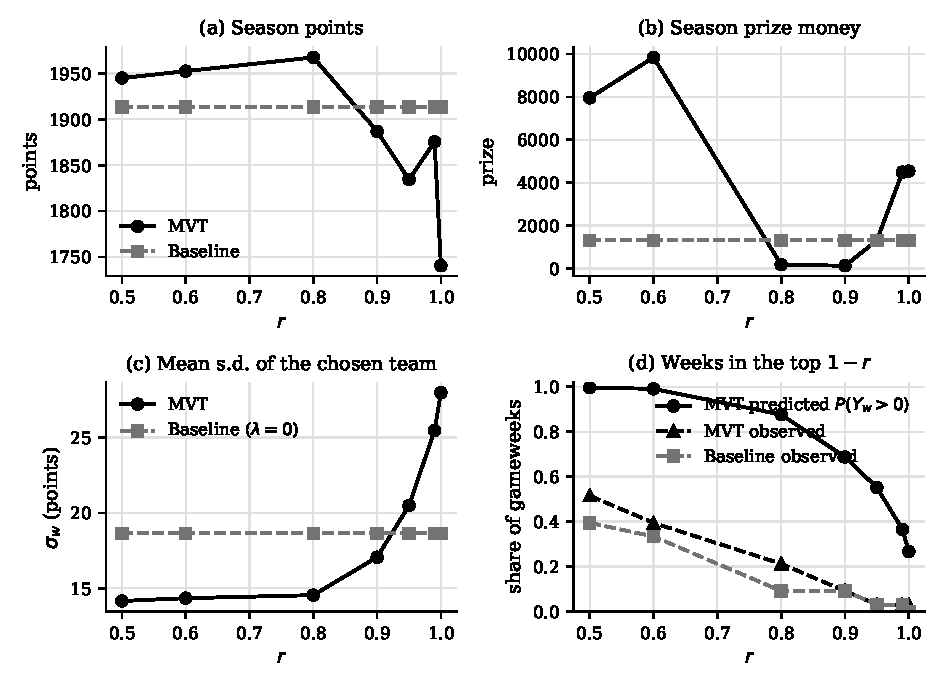
\includegraphics[width=\textwidth]{figures/s1_r_effect.pdf}
		\caption{Stage 1: the effect of $r$. (a) Season points; (b) season prize money; (c) mean
			standard deviation of the chosen team's points; (d) share of gameweeks in the top $1-r$ of the
			real contest, with MVT's mean estimated $\mathrm{Prob}\{Y_w>0\}$.}
		\label{fig:s1-r}
	\end{figure}

	\paragraph{The branch of (3.17) and the variance of the team.} The effect of $r$ runs through
	the branch of Theorem~3.2.3.1. For $r\le 80\%$ the $\lambda=0$ team's mean exceeded
	$\mu_{G^{(r')}}$ in every gameweek, so every week was on the convex branch, and a positive
	$\lambda$ penalises variance: the chosen team's standard deviation fell from 18.64 points for
	the baseline to between 14.16 and 14.55. At $r=90\%$ one gameweek was on the nonconvex branch,
	at $r=95\%$ fifteen, and at $r=99\%$ and $100\%$ all 33. There a positive $\lambda$ rewards
	variance, and the chosen team's standard deviation rose to 20.49, 25.46 and 27.97 points.
	MVT thus does what Theorem~3.2.3.1 prescribes: it buys safety when it expects to be ahead of the
	benchmark and buys variance when it expects to be behind. The size of $\lambda^*$ is not
	comparable across the two branches, because the variance enters with opposite signs; on the
	nonconvex branch the smallest positive values of $\Lambda$ already change the team.

	The nonconvex MIQP did not always finish within the 30-second limit. The share of solves
	stopped at the limit rises with $r$, from 56 of 264 at $r=50\%$ to 223 of 264 at $r=99\%$ and
	$100\%$. At low $r$ only the values $\lambda\ge 0.1$ hit the limit, but these include the
	values most often chosen as $\lambda^*$ at $r=50\%$ ($0.1$ and $0.2$), so some chosen teams are
	the best found rather than proven optimal on either branch.
	At high $r$ the frontier is therefore built from good, but not provably optimal, teams.

	\paragraph{Points.} For $r\le 80\%$ MVT scored slightly more points than the baseline (1945.0
	to 1967.5 against 1913.5), but the paired differences are small relative to their spread, and
	none is significant (Wilcoxon $p\ge 0.56$). For $r\ge 90\%$ MVT scored fewer points. The
	difference is significant at the 5\% level at $r=95\%$ ($-2.39$ points per gameweek, $p=0.015$)
	and at $r=100\%$ ($-5.24$, $p=0.042$), but neither survives a Bonferroni correction for the
	seven values of $r$ (threshold $0.007$). The loss of mean points at high $r$ is the price of the
	variance that MVT deliberately buys on the nonconvex branch.

	\paragraph{Hits and prizes.} At $r=50\%$ MVT finished in the top half of the contest in 17
	gameweeks against the baseline's 13, and at $r=80\%$ in the top fifth in 7 against 3. Neither
	difference is significant (sign test on the discordant gameweeks, $p=0.42$ and $p=0.22$). At
	$r\ge 90\%$ both optimizers hit the target at most three times in 33 gameweeks, and MVT won one
	contest at $r=100\%$, which the baseline never did. Prize money is dominated by single
	gameweeks: of MVT's 7{,}955.61 at $r=50\%$, 7{,}832.38 came from gameweek 24, and of 9{,}841.08 at
	$r=60\%$, 9{,}692.98 from gameweek 23; the baseline earned 1{,}204.85 of its 1{,}303.81 in
	gameweek 26. With a handful of paid gameweeks per season, prize totals cannot separate the two
	optimizers, and we do not test them.

	\paragraph{Calibration.} MVT's estimates of $\mathrm{Prob}\{Y_w>0\}$ are far too high.
	Table~\ref{tab:s1-calibration} pools the 231 team-gameweeks over every $r$ and compares the
	estimate with the observed hit rate in the real contest. In the 69 cases where MVT estimated a
	probability of at least 0.95 (mean 0.994), the team hit its target in 43\% of them; where it
	estimated between 0.2 and 0.4 it hit in 2\%. At $r=50\%$ the mean estimate was 0.996, against an
	observed 17 of 33 (Brier score 0.483). Three causes contribute, each identified above: the
	simulated field is weaker than the real one (Table~\ref{tab:s1-field}), $\mu_\delta$ overstates
	the points of the top players that MVT selects, and $\Sigma_\delta$ rests on few gameweeks of
	errors. The ordering of the estimates is nevertheless informative: the observed rate rises
	with the estimate above 0.4.

	\begin{table}[ht]
		\centering
		\caption{Stage 1: calibration of MVT's estimated $\mathrm{Prob}\{Y_w>0\}$, all $r$ pooled
			(231 team-gameweeks).}
		\label{tab:s1-calibration}
		\begin{tabular}{lrrr}
			\toprule
			Estimate & $n$ & Mean estimate & Observed hit rate \\
			\midrule
			$[0.00, 0.20)$ & 3  & 0.189 & 0.333 \\
			$[0.20, 0.40)$ & 53 & 0.300 & 0.019 \\
			$[0.40, 0.60)$ & 39 & 0.499 & 0.000 \\
			$[0.60, 0.80)$ & 34 & 0.680 & 0.118 \\
			$[0.80, 0.95)$ & 33 & 0.865 & 0.212 \\
			$[0.95, 1.00)$ & 69 & 0.994 & 0.435 \\
			\bottomrule
		\end{tabular}
	\end{table}

	\paragraph{Summary of Stage 1.} The implementation reproduces the qualitative behaviour of the
	method of~\cite{haugh2021}: the branch of (3.17) follows $r$, MVT reduces variance at low $r$
	and increases it at high $r$, and the deliberate variance at high $r$ costs mean points. In a
	single season of 33 contests none of the gains in points or hits at low $r$ is significant,
	and the absolute probability estimates are not calibrated against the real contest.

	\section{Stage 2: The H2H League}
	\label{sec:s2}

	\subsection{Setting}
	\label{sec:s2-setting}

	Stage~2 uses the full FPL rules of §3.1.2: a 15-man squad (2 goalkeepers, 5 defenders, 5
	midfielders, 3 forwards) within the squad's value plus the money in the bank, at most three
	players per club, a starting XI in a valid formation with a doubled captain, and free transfers
	that are banked from week to week. The rolling season starts from our real squad before
	gameweek 6 and then carries the simulated squad, free-transfer bank and money in the bank
	forward. Each gameweek is scored as a real H2H match: the starting XI with the captain doubled,
	with FPL's automatic substitutions and vice-captain rule, against the real opponent's real
	points. The data contain squads but not line-ups, so the XI and captain of every squad not
	chosen by the MIQP (the opponent's sampled squads, a held squad, the real squads) are picked by
	the same rule: the highest predicted xP in a valid formation.

	\paragraph{Points distribution.} The predictor targets xP, so its residuals are xP minus
	prediction. These residuals form the covariance part of $\Sigma_\delta$, built as in
	Section~\ref{sec:design-baseline}. A gameweek is won on points, however, and points scatter
	around xP by about three times as much as xP around the prediction. The variance of realised
	points about xP, pooled per position over past player-gameweeks, is therefore added to the
	diagonal of $\Sigma_\delta$. The gameweeks without an xP target drop out of the residuals.

	\paragraph{The two optimizers.} The baseline solves the $\lambda=0$ problem each week, which is
	the convex branch whatever the opponent: the squad, XI and captain with the highest predicted
	xP within the budget and free transfers. It transfers when the new squad adds more than 0.01
	predicted points to holding. MVT solves the MIQP over the grid $\Lambda=\{0\}\cup\{$ten values
	spaced geometrically from 0.01 to 5$\}$, with 20{,}000 opponent squad draws and 2{,}000 Monte
	Carlo draws of $(\delta,G^{(r')})$, and transfers only if the best squad's estimated
	$\mathrm{Prob}\{Y_w>0\}$ exceeds that of holding by 0.03; otherwise it holds, and $\lambda^*$
	is undefined for that week. Both use the same seed (42). For all seven MVT seasons the MIQP time
	limit is 60 seconds per $\lambda$; the baseline keeps the 30 seconds of the original runs, which
	does not bind on the convex branch.

	\subsection{The opponent model}
	\label{sec:s2-opponent}

	\paragraph{The league baseline and the manager fits.} The league Dirichlet-multinomial model
	(3.2)--(3.3) was refitted for every gameweek from 6 to 38 and every position, 132 fits. All
	converged: maximum $\hat R=1.01$, minimum bulk effective sample size 1{,}631, and no divergent
	transitions. The manager-level update (3.4)--(3.5) was fitted for each gameweek's opponent, on
	between 2 and 34 weeks of that manager's history, again 132 fits (maximum $\hat R=1.01$, minimum
	bulk effective sample size 1{,}718). Of these, 28 had divergent transitions, 63 in all and at
	most 6 in one fit; 17 of the 28 are defender fits. With effective sample sizes this high, a
	handful of divergences does not invalidate the posterior means we use, but it marks the
	defender fits as the least well-behaved.
	The retention coefficient $\gamma_m$ is large throughout: its posterior mean ranges from 2.32 to
	10.07, with median 5.3, so a player the manager already owns has his Dirichlet weight
	multiplied by $e^{\gamma_m}$, a factor of at least 10. The model has learned what transfer rules
	and habit imply, that managers mostly keep their squads.

	\paragraph{Overhaul weeks.} A week in which a manager replaces 8 or more of the 15 players is
	treated as a Wildcard or Free Hit and is excluded from that manager's history. League-wide, 77
	manager-weeks were detected, involving all 20 managers. Most come in clusters that are
	implausible as individual decisions: in gameweeks 35 and 36, 19 of the 20 managers are flagged.
	The league data show why. Every manager's recorded squad of gameweek 34 shares a median of 2 of
	15 players with his gameweek 33 squad and 3 with his gameweek 35 squad, while the gameweek 33 and
	35 squads share a median of 13.5. The gameweek 34 squads are therefore a recording error in
	the league data, not chips. Similar league-wide breaks occur between gameweeks 5 and 6 and
	between 29 and 31, where the median overlap of consecutive squads falls to 4.5 and 3 of 15; we
	cannot tell from the data whether these are errors or real. The overhaul filter removes all
	of these weeks from the histories, so the selection model is not trained on them.

	\subsection{The sparse C-vine}
	\label{sec:s2-vine}

	Section~3.2.2 specifies a C-vine over the pool of $M$ players (here the 30 most likely
	players per position, $M=120$), truncated at tree 15, with each pair-copula chosen by AIC from
	six families. The implementation uses a sparse vine instead: Gaussian pair-copulas only, chosen
	by BIC, a single tree, pairs with $|\tau|$ below 0.35 set to independence, and only the players
	who appear in the manager's history (between 11 and 32 per week) entering the vine. To show why,
	we fitted both vines in every gameweek from 6 to 38, on the opponent's latent uniforms $U$
	(eqs.~(3.6)--(3.7)) and on a copy of $U$ with each column permuted independently, which destroys
	any dependence between players while keeping the marginals. We also recorded the mean held-out
	log-likelihood of the last 4, 6 and 8 weeks under a vine fitted on the earlier weeks;
	independence scores exactly 0 on this measure. Table~\ref{tab:s2-vine} summarises the results.

	\begin{table}[ht]
		\centering
		\caption{Stage 2: vine diagnostics over the 33 gameweeks of the rolling season. Held-out
			log-likelihoods are available in 27 gameweeks (at least five weeks of history must remain).}
		\label{tab:s2-vine}
		\begin{tabular}{lrr}
			\toprule
			& Chapter 3 vine & Sparse vine \\
			\midrule
			Dimension                                   & 120 & 11--32 \\
			Non-independent pairs, real $U$ (mean)      & 378.0 & 0.09 \\
			Non-independent pairs, permuted $U$ (mean)  & 383.2 & --- \\
			Gameweeks with more pairs on permuted $U$   & 22 & --- \\
			Log-likelihood, real $U$ (mean)             & 762.7 & 0.20 \\
			Log-likelihood, permuted $U$ (mean)         & 766.9 & 0.21 \\
			Held-out log-likelihood $<0$ (gameweeks)    & 22 of 27 & 4 of 27 \\
			Held-out log-likelihood, median             & $-957.9$ & 0.0 \\
			\bottomrule
		\end{tabular}
	\end{table}

	\paragraph{The Chapter 3 vine fits noise.} With the six families and AIC over 120 players, the
	vine finds as much dependence in the permuted data as in the real data: on average 378 of its
	1{,}680 pairs are non-independent on the real $U$ and 383 on the permuted $U$, with more on the
	permuted data in 22 of the 33 gameweeks, and its in-sample log-likelihood is no higher on the
	real data (762.7 against 766.9). On held-out weeks it scores below independence in 22 of the 27
	gameweeks where the measure is defined, with a median of $-957.9$, and the held-out
	log-likelihood is $-\infty$ in 7 of them: the fitted pair-copulas put zero density where later
	weeks fall. With a manager history of 4 to 33 weeks and 120 players, AIC has too little data to
	reject the flexible families, and the fitted dependence is overfitting. In the first seven
	gameweeks, with 4 to 9 weeks of history, every pair falls back to independence.

	\paragraph{The sparse vine reduces to independence.} The sparse vine fits no non-independent
	pair in 30 of the 33 gameweeks and one pair in each of the other three. Its log-likelihood is
	not distinguishable from its permutation null (mean 0.20 against 0.21), it exceeds the null in
	only 2 gameweeks, and its held-out log-likelihood is zero in 22 gameweeks, negative in 4 and
	positive in 1 (0.17). The data therefore contain no dependence between an opponent's player
	choices that a vine can detect beyond the marginals. This is a finding about the data, not a
	failure of the software: a manager's history is short, most players are held unchanged for
	weeks (so their latent uniforms are draws within one interval of (3.7)), and the transfers that
	do occur are too few to estimate pairwise dependence among dozens of players. For §3.2.2 this
	means that, with one season of one manager's squads, the copula step adds nothing to the
	marginals of §3.2.1. The squads in $\mathbb{W}_o$ are, in effect, drawn from independent
	positional marginals and then filtered by the squad rules, the opponent's free transfers and
	squad value. The dependence that real squads do have, through the budget, the club limit and
	the transfer limit, enters through that filter rather than through the copula.

	\paragraph{The size of $\mathbb{W}_o$.} Of the 20{,}000 draws per gameweek, between 7{,}052 and
	18{,}327 were feasible squads, and these contained between 124 and 10{,}406 distinct squads
	(median 2{,}751). $\mathbb{W}_o$ is small in weeks when the opponent had a single free transfer,
	since most feasible draws then repeat the current squad with one change.

	\subsection{A worked gameweek}
	\label{sec:s2-worked}

	To show how one decision is made, we take the gameweek of the $r=50\%$ season in which a
	positive $\lambda^*$ gained most in estimated $\mathrm{Prob}\{Y_w>0\}$ over $\lambda=0$. This is
	gameweek 9, against manager 593532. Of the 20{,}000 opponent draws, 15{,}959 were feasible
	squads, and these contained 1{,}763 distinct squads. Over the Monte Carlo draws the benchmark
	$G^{(r')}$ had mean 61.76 and standard deviation 6.68 points. Our current squad's predicted
	mean exceeded $\mu_{G^{(r')}}$ by 4.86 points, so the week was on the convex branch of (3.17).

	\begin{figure}[ht]
		\centering
		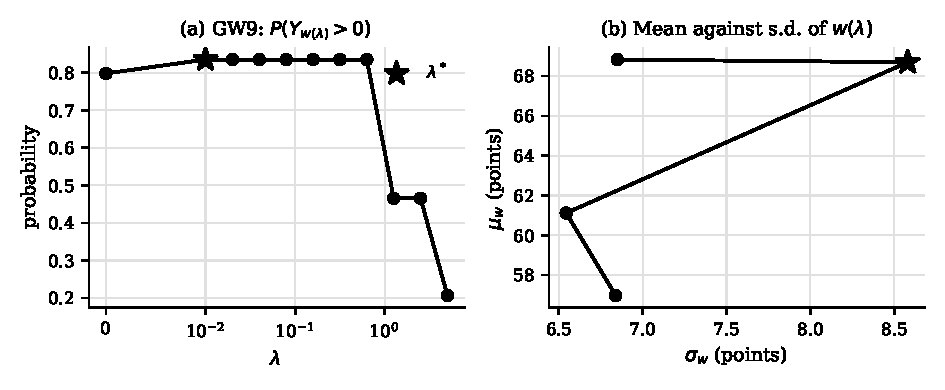
\includegraphics[width=\textwidth]{figures/s2_frontier.pdf}
		\caption{Stage 2, gameweek 9 at $r=50\%$: (a) estimated $\mathrm{Prob}\{Y_{w(\lambda)}>0\}$
			over $\Lambda$, with $\lambda^*$ marked; (b) predicted mean against standard deviation of the
			teams $w(\lambda)$.}
		\label{fig:s2-frontier}
	\end{figure}

	Figure~\ref{fig:s2-frontier} shows the frontier. The grid produced only four distinct teams. At
	$\lambda=0$ the team had mean 68.83 and standard deviation 6.85 points, with estimated
	$\mathrm{Prob}\{Y_w>0\}=0.798$. Every $\lambda$ from 0.01 to 0.63 gave a second team, with mean
	68.69, standard deviation 8.58 and estimated probability 0.835. Larger values gave weaker
	teams: mean 61.12 and probability 0.466 at $\lambda=1.26$ and $2.51$, and mean 56.98 and
	probability 0.207 at $\lambda=5$. MVT therefore chose $\lambda^*=0.01$ and made one transfer.

	The chosen team has a higher variance of its own than the $\lambda=0$ team, although the week
	is on the convex branch. This is consistent with (3.17), because on the convex branch $\lambda$
	penalises the variance of the difference $Y_w$, not of our team. That variance falls when our
	points covary with $G^{(r')}$, that is, when we hold players the opponent is likely to hold.
	For the $\lambda=0.01$ team to be preferred, its covariance with $G^{(r')}$ must have risen by
	more than its own variance. In the H2H setting, MVT ahead of the benchmark protects its lead
	by matching the opponent rather than by choosing low-variance players. The protection did not
	pay off in this week: MVT scored 66 points and the baseline 70, and the opponent's 73 beat both.

	\subsection{MVT against the baseline over the season}
	\label{sec:s2-season}

	We first compare the two optimizers at $r=50\%$. There the benchmark is the median of the
	opponent's simulated squads, so $\mathrm{Prob}\{Y_w>0\}$ is the closest analogue of the
	probability of winning the match. Both optimizers solved all 33 gameweeks. The $\lambda=0$
	problem was solved to optimality in every week. Of the 363 MIQP solves of the MVT season, 166
	stopped at the 60-second limit, all of them at $\lambda>0$. Figure~\ref{fig:s2-season} shows
	the cumulative points of both optimizers, our real team and its real opponents.

	\begin{figure}[ht]
		\centering
		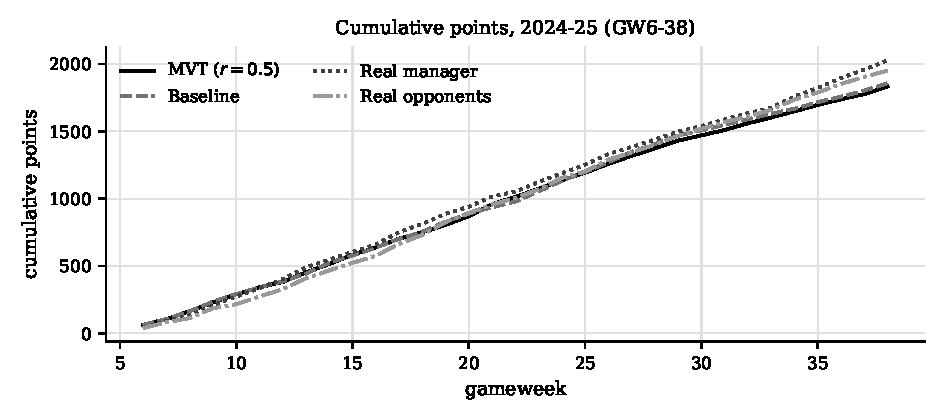
\includegraphics[width=\textwidth]{figures/s2_season.pdf}
		\caption{Stage 2: cumulative points from gameweek 6 to 38 of MVT ($r=50\%$), the baseline,
			our real team and its real opponents, all scored with the same line-up rule.}
		\label{fig:s2-season}
	\end{figure}

	\paragraph{Points, wins and xP.} MVT scored 1{,}833 points and won 12.5 matches, counting ties
	as half a win. The baseline scored 1{,}858 points and won 11. The paired difference in points
	is $-0.76$ per gameweek, with a 95\% bootstrap interval of $[-4.36, 3.24]$ (Wilcoxon $p=0.35$,
	$n=27$ gameweeks with a non-zero difference). The two optimizers' match results differ in only
	4 gameweeks: MVT won 3 of them and the baseline 1 (sign test $p=0.63$). MVT's teams had lower
	predicted xP: 67.69 points per gameweek against 71.80, over the 30 gameweeks with an xP target.
	Both optimizers made one transfer in every gameweek, and MVT never held. Neither optimizer
	comes near our real team. Scored with the same line-up rule, it made 2{,}027 points and won 21
	matches, while its real opponents made 1{,}950.

	\paragraph{The choice of $\lambda^*$.} In 23 of the 33 gameweeks our current squad's predicted
	mean was below $\mu_{G^{(r')}}$, so the week was on the nonconvex branch even at $r=50\%$. The
	real opponents' squads were, on the predictions, mostly stronger than ours. $\lambda^*$ was 0
	in 23 gameweeks, 0.01 in 7, 0.079 in 2 and 0.158 in 1. Of the ten positive values, six were on
	the convex branch and four on the nonconvex branch. The chosen team's standard deviation
	averaged 10.53 points, against the baseline's 9.77.

	\paragraph{Calibration.} MVT's mean estimated $\mathrm{Prob}\{Y_w>0\}$ was 0.62, against an
	observed win rate of 0.38 (Brier score 0.382). The estimates are therefore too high, as in
	Stage~1, though by less: the opponent model describes a single real manager, while the
	simulated field of Stage~1 was weaker than the real contest. The upward bias of $\mu_\delta$ for
	the top-predicted players (Section~\ref{sec:predictions}) applies here as well.

	\subsection{The effect of $r$}
	\label{sec:s2-r}

	The MVT season was run at $r\in\{50,60,80,90,95,99,100\}\%$ against the same baseline.
	Table~\ref{tab:s2-r} and Figure~\ref{fig:s2-r} report the results. Every season solved all 33
	gameweeks, and no gameweek needed the single-squad fallback. The $\lambda=0$ problem was solved
	to optimality in every gameweek except one: at $r=99\%$, gameweek 38 stopped at the time limit
	and kept its best team found. Between 145 and 187 of each season's 363 solves stopped at the
	60-second limit, so at $\lambda>0$ the frontier consists of the best teams found, not proven
	optima. At $r=100\%$ the benchmark equalled the maximum over $\mathbb{W}_o$ in every draw of
	every gameweek, as intended.

	\begin{table}[ht]
		\centering
		\caption{Stage 2: MVT at each $r$ against the baseline, 33 gameweeks. Nonconvex: gameweeks on
			the nonconvex branch of (3.17). $\sigma_w$: mean standard deviation of the chosen team's points
			under $\Sigma_\delta$. $\Delta$ points: mean difference per gameweek (MVT minus baseline) with a
			95\% bootstrap interval; $p$: Wilcoxon signed-rank test. Wins count ties as 0.5; $p_W$: sign
			test on the gameweeks where the two match results differ. $\hat P$: mean estimated
			$\mathrm{Prob}\{Y_w>0\}$.}
		\label{tab:s2-r}
		\footnotesize
		\setlength{\tabcolsep}{3pt}
		\begin{tabular}{rrrrrrrrrrr}
			\toprule
			$r$ & Nonconvex & $\lambda^*\neq0$ & Held & $\sigma_w$ & Points & $\Delta$ points [95\% CI] & $p$ & Wins & $p_W$ & $\hat P$ \\
			\midrule
			50\%  & 23 & 10 & 0 & 10.53 & 1833 & $-0.76$ [$-4.36$, $3.24$] & 0.348 & 12.5 & 0.625 & 0.622 \\
			60\%  & 21 & 13 & 0 &  9.30 & 1822 & $-1.09$ [$-5.42$, $3.12$] & 0.559 & 12.5 & 0.625 & 0.550 \\
			80\%  & 22 &  9 & 0 & 10.27 & 1881 & $+0.70$ [$-2.09$, $3.67$] & 0.880 & 13.5 & 0.250 & 0.557 \\
			90\%  & 27 & 11 & 0 & 10.23 & 1891 & $+1.00$ [$-1.97$, $4.21$] & 0.776 & 13.0 & 0.250 & 0.478 \\
			95\%  & 28 & 13 & 0 & 10.33 & 1902 & $+1.33$ [$-1.48$, $4.30$] & 0.546 & 12.5 & 0.500 & 0.430 \\
			99\%  & 33 & 20 & 0 & 12.12 & 1775 & $-2.52$ [$-7.48$, $2.52$] & 0.335 & 16.0 & 0.039 & 0.247 \\
			100\% & 33 & 18 & 5 & 11.56 & 1702 & $-4.73$ [$-8.45$, $-1.00$] & 0.017 & 10.0 & 1.000 & 0.158 \\
			\midrule
			Baseline & 0 & --- & 0 & 9.77 & 1858 & --- & --- & 11.0 & --- & --- \\
			\bottomrule
		\end{tabular}
	\end{table}

	\begin{figure}[ht]
		\centering
		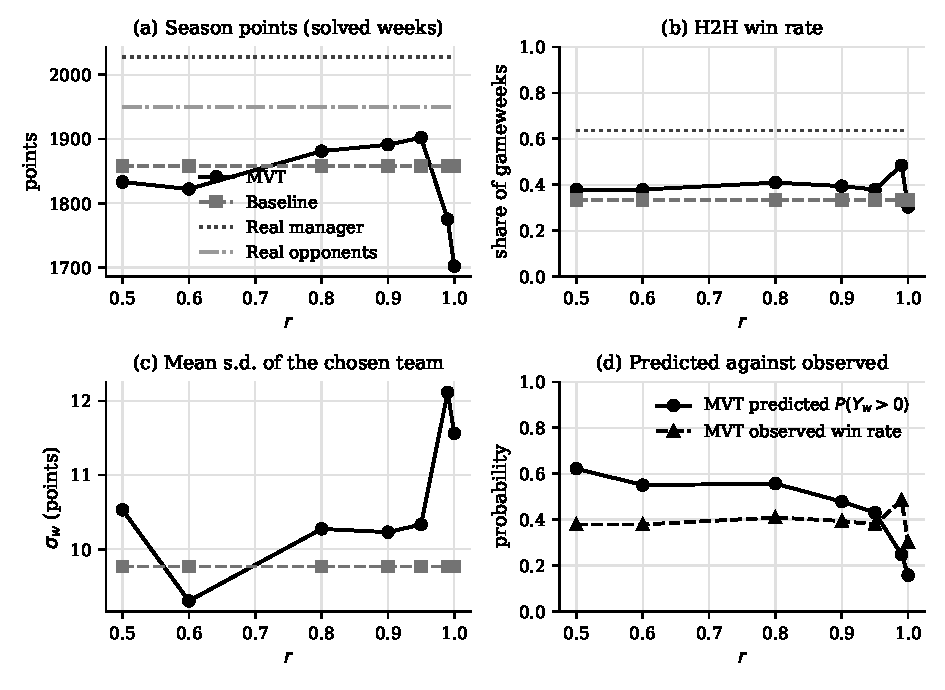
\includegraphics[width=\textwidth]{figures/s2_r_effect.pdf}
		\caption{Stage 2: the effect of $r$. (a) Season points; (b) H2H win rate; (c) mean standard
			deviation of the chosen team's points; (d) MVT's mean estimated $\mathrm{Prob}\{Y_w>0\}$ and
			observed win rate.}
		\label{fig:s2-r}
	\end{figure}

	\paragraph{The branch and the variance of the team.} As in Stage~1, the branch of (3.17)
	follows $r$. Between 21 and 23 gameweeks were on the nonconvex branch for $r\le 80\%$, 27 and
	28 at $r=90\%$ and $95\%$, and all 33 at $r=99\%$ and $100\%$. Unlike Stage~1, most weeks are on
	the nonconvex branch even at low $r$, because the opponents' squads were predicted to be
	stronger than ours. $\lambda^*$ was 0 in 20 to 24 gameweeks for $r\le 95\%$ and positive in 20
	and 18 at $r=99\%$ and $100\%$. At $r=100\%$ MVT also held its squad in 5 gameweeks, where no
	team improved on holding by the 0.03 margin. The chosen team's standard deviation is close to
	the baseline's for $r\le 95\%$ (9.30 to 10.53 against 9.77) and higher at $r=99\%$ and $100\%$
	(12.12 and 11.56). MVT does not reduce the team's variance at low $r$ as it did in Stage~1, for
	two reasons. Most weeks are on the nonconvex branch. On the convex branch, the variance that
	(3.17) penalises is that of the difference with the opponent, which can fall while our team's
	own variance rises (Section~\ref{sec:s2-worked}).

	\paragraph{Points.} No value of $r$ gives MVT significantly more points than the baseline. The
	differences for $r\le 95\%$ lie between $-1.09$ and $+1.33$ points per gameweek, with
	Wilcoxon $p\ge 0.35$. At $r=100\%$ MVT scored 4.73 points per gameweek fewer ($p=0.017$, $n=31$),
	and at $r=99\%$ 2.52 fewer ($p=0.34$). As in Stage~1, the variance bought on the nonconvex
	branch costs mean points. Like Stage~1's significant results, $p=0.017$ does not survive a
	Bonferroni correction for the seven values of $r$ (threshold 0.007).

	\paragraph{Wins.} MVT won between 12.5 and 13.5 matches for $r\le 95\%$, against the baseline's
	11. Its match results differed from the baseline's in at most 3 gameweeks, so none of these
	differences can be significant. The most wins came at $r=99\%$: 16 against 11, with MVT winning
	8 of the 9 discordant gameweeks (sign test $p=0.039$), despite scoring 83 fewer points over the
	season. At $r=100\%$ MVT won 10. A higher-variance team can win more often while scoring fewer
	points in total, and (3.17) aims at exactly this trade-off. However, the $r=99\%$ result does not
	survive the Bonferroni correction, the neighbouring values of $r$ do not show it, and one season
	of 33 matches cannot separate it from chance.

	\paragraph{Calibration.} For $r>50\%$ the benchmark lies above the median of the opponent's
	squads, so $\mathrm{Prob}\{Y_w>0\}$ is a probability of beating a stronger squad than the
	opponent's typical one, not of winning the match. The mean estimate falls with $r$, from 0.62
	to 0.16, while the observed win rate stays between 0.30 and 0.48. The estimate is above the win
	rate for $r\le 95\%$ and below it at $r=99\%$ and $100\%$, as the stricter benchmark implies.

	\section{Discussion}
	\label{sec:discussion}

	\paragraph{MVT against the baseline.} The two stages agree on how MVT behaves and on what it
	achieves. In both, the branch of (3.17) follows $r$, and MVT buys variance when it expects to be
	behind the benchmark. In both, that variance costs mean points at $r=100\%$: $-5.24$ points per
	gameweek in Stage~1 and $-4.73$ in Stage~2. In neither stage does MVT score significantly more
	points than the baseline at any $r$, or hit its target significantly more often once the
	seven values of $r$ are accounted for. MVT's estimated probabilities are too high at $r=50\%$ in
	both stages, far more so in Stage~1 (0.996 against an observed 0.52) than in Stage~2 (0.62
	against 0.38). With 33 gameweeks per stage, the method's advantage over a points maximiser, if
	it exists, is smaller than one season can detect.

	\paragraph{Winner-takes-all against lower $r$.} In a FantasyGo contest, $r$ is set by the
	payout: a team must finish in the top $1-r$ of a field of hundreds to be paid, and the field's
	quantile is the natural benchmark. At low $r$ our team is usually ahead of that benchmark, and
	MVT buys safety; in a winner-takes-all contest ($r=100\%$) it must beat the best entry, is
	always behind, and buys variance. An H2H match has no field. The match is won by beating one
	opponent, and the benchmark that represents this most directly is $r=50\%$, the median of the
	opponent's possible squads. A higher $r$ asks MVT to beat the opponent's best plausible squad,
	a stricter target than the match requires. It moves every week to the nonconvex branch, and at
	$r=100\%$ it cost points without adding wins. In H2H, $r$ is therefore not dictated by the
	rules but acts as a risk setting. The single season suggests that a high setting ($r=99\%$) may
	convert variance into wins, but the evidence is not strong enough to recommend it.

	\paragraph{Non-strategic opponents.} The opponents in both stages are modelled from their own
	past behaviour, and our choice does not enter $\mathbb{W}_o$. In a FantasyGo contest with
	hundreds of entries this is close to true: no single entry can track and respond to ours. In an
	H2H league it is an approximation. Each manager knows his opponent in advance and can see that
	opponent's squad from previous gameweeks. A strategic opponent could respond to our expected
	squad, for example by doubling our likely captain to cancel his points or by avoiding our
	players to create variance. The model would then misstate both the location of $G^{(r')}$ and
	its covariance $\sigma_{\delta,G^{(r')}}$ with our players, which is the term through which
	(3.17) decides whether to copy or avoid the opponent's players. The stability of the squads we
	observe ($\gamma_m$ between 2.32 and 10.07) suggests that, in this league, managers mostly
	manage their own squads rather than respond to opponents. A game-theoretic treatment, as in the
	opponent classification and the ``sword'' and ``shield'' strategies outlined in §1.4, is
	outside what we implemented.

	\paragraph{The objectives of §1.3.2.} (i) The H2H problem was formulated as the mean-variance
	problem of Chapter~3, with the opponent's simulated squads as the benchmark, and solved as a
	MIQP over $\Lambda$ in every gameweek of every season; the $\lambda=0$ problem was solved to
	optimality in all but one gameweek, and the problems at $\lambda>0$ often to the time limit.
	(ii) Player points were predicted per position (Section~\ref{sec:predictions}), with the
	caveat that the predictions overstate the points of the top-predicted players. (iii) The
	opponents' squads were modelled by the league and manager selection models, which converged;
	the copula step reduced to independence, so the squads are drawn from the positional
	marginals filtered by the squad rules. (iv) The rolling season produced a transfer, starting
	XI and captain in every gameweek. (v) On 2024-25 FPL data the method showed no significant
	advantage over the baseline in points or wins. Both optimizers stayed well below our real
	team (2{,}027 points and 21 wins, against between 1{,}702 and 1{,}902 points and between 10 and
	16 wins), which points to the predictions, rather than the optimization, as the main
	limitation.

	\paragraph{Limitations.} Each stage is a single season of 33 gameweeks, so paired tests have
	little power, and a handful of contests decide the prize totals. $\Sigma_\delta$ rests on at
	most 33 gameweeks of errors for several hundred players; its correlations are noisy, and the
	eigenvalue floor keeps it usable without making it accurate. $\mu_\delta$ overstates the
	realised points of the top-predicted players by about one point per player
	(Section~\ref{sec:predictions}), which makes every estimated probability optimistic. The
	opponent model does not include chips: Wildcard and Free Hit weeks are excluded from the
	histories, but our model does not predict when an opponent will play one. The league data
	contain an erroneous gameweek of squads (gameweek 34) and two league-wide breaks of unknown
	origin. In Stage~2 the two optimizers' match results differ in at most 9 of the 33 gameweeks,
	so every comparison of wins rests on a handful of matches. Between 145 and 187 of each MVT
	season's 363 solves stopped at the 60-second limit, nearly all at $\lambda>0$, so those teams
	are the best found rather than proven optima. Because the limit is in wall-clock time, a run on a loaded machine can return
	different teams; the baseline reported here was run alone and reproduces the original
	baseline's decisions exactly. Finally, our line-ups and those of the opponents and our real
	team are all chosen by the same rule, so the comparison is fair, but the real managers'
	line-up decisions are not modelled.



	\appendix
	%\begin{table}[H]
	%	\begin{center}
	%		\begin{tabular}{|c|}
	%			\hline
	%			Gaussian (or Normal) copula ( $-1 \le \theta \le 1$ ) \\
	%			\hline
	%			\(\begin{aligned}
	%					C\left(u_1,u_2; \theta \right) &= \Phi_2 \left(\Phi^{-1} \left(u_1\right), \Phi^{-1} left(u_2\right)\right) \\
	%					c\left(u_1,u_2; \theta \right) &= \frac{1}{\sqrt{1-\theta^2}} \exp \left{
	%					- \frac{\theta^2 \left(w^2_1 + w^2_2\right) - 2\theta w_1 w_2}{2\left(1-\theta^2\right)}
	%					}, \text{where} w_1 = \Phi^{-1}\left(u_1\right), w_2 = \Phi_{-1}\left(u_2\right)
	%
	%				\end{aligned}\)
	%
	%			\hline
	%			dj\\
	%
	%
	%			\hline
	%			0.143 \\
	%			\hline
	%		\end{tabular}
	%	\end{center}
	%	\caption{Mean-variance frontier for the game week-38 worked example ($r=80\%$); the starred row is $\lambda^*=\argmax_\lambda \widehat{Prob}(Y_{w(\lambda)}>0)$.}
	%	\label{tab:copula_definitions}
	%\end{table}
		\begin{table}[H]
			\centering
			\renewcommand{\arraystretch}{1.4}
			\begin{tabular}{|c|}
				\hline

				\textbf{Gaussian (Normal) copula}
				$\left(-1 < \theta < 1\right)$
				\\
				\hline

				\(\begin{aligned}
					C(u,v;\theta) &= \Phi_2\left( \Phi^{-1}(u),\Phi^{-1}(v);\theta \right), \\[2pt]

					c(u,v;\theta) &= \frac{1}{\sqrt{1-\theta^2}} \exp\left\{ \frac{ \theta^2(w_1^2+w_2^2)-2\theta w_1w_2 }{ 2(1-\theta^2)} \right\},  \\[2pt]

					h(u|v;\theta) &= \Phi\left( \frac{ \Phi^{-1}(u)-\theta\Phi^{-1}(v) }{ \sqrt{1-\theta^2} }\right),\\[2pt]


					h^{-1}(u|v;\theta)
					&=
					\Phi\left[
					\theta\Phi^{-1}(v)
					+
					\sqrt{1-\theta^2}\Phi^{-1}(u)
					\right],\\[2pt]

					&\qquad
					w_1=\Phi^{-1}(u),\quad
					w_2=\Phi^{-1}(v).
				\end{aligned}\)

				\\
				\hline


				\textbf{Student-$t$ copula}
				$\left(-1 < \theta < 1,\;\nu>0\right)$
				\\
				\hline

				\(\begin{aligned}
					C(u,v;\theta,\nu)
					&=
					t_{2,\theta,\nu}
					\left(
					t_\nu^{-1}(u),t_\nu^{-1}(v)
					\right),\\[2pt]
					c(u,v;\theta,\nu)
					&=
					\frac{
						\Gamma\left(\frac{\nu+2}{2}\right)
					}{
						\Gamma\left(\frac{\nu}{2}\right)
						\pi\nu\sqrt{1-\theta^2}
					}
					\frac{
						\left[
						1+
						\frac{
							w_1^2-2\theta w_1w_2+w_2^2
						}{
							\nu(1-\theta^2)
						}
						\right]^{-\frac{\nu+2}{2}}
					}{
						\left(1+\frac{w_1^2}{\nu}\right)^{-\frac{\nu+1}{2}}
						\left(1+\frac{w_2^2}{\nu}\right)^{-\frac{\nu+1}{2}}
					},\\[2pt]
					h(u|v;\theta,\nu)
					&=
					T_{\nu+1}\left(
					\frac{
						w_1-\theta w_2
					}{
						\sqrt{
							(1-\theta^2)
							\frac{\nu+w_2^2}{\nu+1}
						}
					}
					\right),\\[2pt]

					h^{-1}(u|v;\theta,\nu)
					&=
					T_\nu\left[
					\theta w_2+
					\sqrt{
						(1-\theta^2)
						\frac{\nu+w_2^2}{\nu+1}
					}
					T_{\nu+1}^{-1}(u)
					\right],\\[2pt]

					&\qquad
					w_1=t_\nu^{-1}(u),\quad
					w_2=t_\nu^{-1}(v).
				\end{aligned}\)

				\\
				\hline


				\textbf{Clayton copula}
				$\left(\theta>0\right)$
				\\
				\hline

				\(\begin{aligned}
					C(u,v;\theta)
					&= max \{ \left(u^{-\theta}+v^{-\theta}-1 \right)^{-1/\theta}, 0 \},\\[2pt]

					c(u,v;\theta)
					&= max \{
					(1+\theta)
					(uv)^{-(1+\theta)}
					\left(
					u^{-\theta}+v^{-\theta}-1
					\right)^{-2-\frac{1}{\theta}}, 0 \},\\[2pt]

					h(u|v;\theta)
					&= max \{
					v^{-\theta-1}
					\left(
					u^{-\theta}+v^{-\theta}-1
					\right)^{-1/\theta-1}, 0 \},\\[2pt]

					h^{-1}(u|v;\theta)
					&=
					\left[
					1+
					v^{-\theta}
					\left(
					u^{-\frac{\theta}{1+\theta}}-1
					\right)
					\right]^{-1/\theta}.\\[2pt]
				\end{aligned}\)

				\\
				\hline


				\textbf{Gumbel copula}
				$\left(\theta\geq1\right)$
				\\
				\hline

				\(\begin{aligned}
					C(u,v;\theta)
					&=
					\exp\left\{
					-\left[
					(-\log u)^\theta+
					(-\log v)^\theta
					\right]^{1/\theta}
					\right\},\\[2pt]
					c(u,v;\theta)
					&=
					\frac{C(u,v;\theta)}{uv}
					\left[
					(-\ln u)^\theta+
					(-\ln v)^\theta
					\right]^{\frac{2}{\theta}-2}\\
					&\quad\times
					(-\ln u)^{\theta-1}
					(-\ln v)^{\theta-1}
					\left[
					1+
					(\theta-1)
					\left(
					(-\ln u)^\theta+
					(-\ln v)^\theta
					\right)^{-1/\theta}
					\right],\\[2pt]
					h(u|v;\theta)
					&=
					C(u,v;\theta)
					\frac{
						(-\ln v)^{\theta-1}
					}{
						v
					}
					\left[
					(-\ln u)^\theta+
					(-\ln v)^\theta
					\right]^{\frac{1}{\theta}-1},\\[2pt]
					&\qquad
					h^{-1}(v|u;\theta) \text{ obtained numberically unsing Newton's method}.
				\end{aligned}\)

				\\
				\hline


				\textbf{Frank copula}
				$\left(\theta\neq0\right)$
				\\
				\hline

				\(\begin{aligned}
					C(u,v;\theta)
					&=
					-\frac{1}{\theta}
					\ln\left[
					1+
					\frac{
						(e^{-\theta u}-1)
						(e^{-\theta v}-1)
					}{
						e^{-\theta}-1
					}
					\right],\\[2pt]
					c(u,v;\theta)
					&=
					\frac{
						\theta(1-e^{-\theta})
						e^{-\theta(u+v)}
					}{
						\left[
						(1-e^{-\theta})
						+
						(e^{-\theta u}-1)
						(e^{-\theta v}-1)
						\right]^2
					},\\[2pt]
					h_{1|2}(u|v;\theta)
					&=
					\frac{
						e^{-\theta v}
						(e^{-\theta u}-1)
						+
						e^{-\theta v}
						-
						e^{-\theta}
					}{
						(e^{-\theta u}-1)
						(e^{-\theta v}-1)
						+
						e^{-\theta}-1
					},\\[2pt]
					h_{2|1}(v|u;\theta)
					&=
					\frac{
						e^{-\theta u}
						(e^{-\theta v}-1)
						+
						e^{-\theta u}
						-
						e^{-\theta}
					}{
						(e^{-\theta u}-1)
						(e^{-\theta v}-1)
						+
						e^{-\theta}-1
					}.
				\end{aligned}\)

				\\
				\hline


				\textbf{Independence copula}
				\\
				\hline

				\(\begin{aligned}
					C(u,v)
					&=uv,\\
					c(u,v)
					&=1,\\
					h_{1|2}(u|v)
					&=u,\qquad
					h_{2|1}(v|u)=v,\\
					h^{-1}_{1|2}(q|v)
					&=q,\qquad
					h^{-1}_{2|1}(q|u)=q.
				\end{aligned}\)

				\\
				\hline

			\end{tabular}
			\caption{Bivariate copula families, corresponding copula densities, $h$-functions, and inverse $h$-functions.}
			\label{tab:copula_definitions}
		\end{table}

	\begin{table}[H]
		\centering
		\renewcommand{\arraystretch}{1.3}
		\small
		\begin{tabularx}{\textwidth}{|X|}
			\hline

			\textbf{Gaussian (Normal) copula}
			$\left(-1 < \theta < 1\right)$
			\\ \hline

			\[
			\begin{aligned}
				C(u,v;\theta)
				&= \Phi_2\left(
				\Phi^{-1}(u),\Phi^{-1}(v);\theta
				\right),\\[2pt]
				c(u,v;\theta)
				&=
				\frac{1}{\sqrt{1-\theta^2}}
				\exp\left\{
				\frac{
					\theta^2(w_1^2+w_2^2)-2\theta w_1w_2
				}{
					2(1-\theta^2)
				}
				\right\},\\[2pt]
				h(u|v;\theta)
				&=
				\Phi\left(
				\frac{
					\Phi^{-1}(u)-\theta\Phi^{-1}(v)
				}{
					\sqrt{1-\theta^2}
				}
				\right),\\[2pt]
				h^{-1}(u|v;\theta)
				&=
				\Phi\left[
				\theta\Phi^{-1}(v)
				+
				\sqrt{1-\theta^2}\Phi^{-1}(u)
				\right],\\[2pt]
				&\qquad
				w_1=\Phi^{-1}(u),\quad
				w_2=\Phi^{-1}(v).
			\end{aligned}
			\]

			\\ \hline

			\textbf{Student-$t$ copula}
			$\left(-1 < \theta < 1,\;\nu>0\right)$
			\\ \hline

			\[
			\begin{aligned}
				C(u,v;\theta,\nu)
				&=
				t_{2,\theta,\nu}
				\left(
				t_\nu^{-1}(u),t_\nu^{-1}(v)
				\right),\\[2pt]
				c(u,v;\theta,\nu)
				&=
				\frac{
					\Gamma\left(\frac{\nu+2}{2}\right)
				}{
					\Gamma\left(\frac{\nu}{2}\right)
					\pi\nu\sqrt{1-\theta^2}
				}
				\frac{
					\left[
					1+
					\frac{
						w_1^2-2\theta w_1w_2+w_2^2
					}{
						\nu(1-\theta^2)
					}
					\right]^{-\frac{\nu+2}{2}}
				}{
					\left(1+\frac{w_1^2}{\nu}\right)^{-\frac{\nu+1}{2}}
					\left(1+\frac{w_2^2}{\nu}\right)^{-\frac{\nu+1}{2}}
				},\\[2pt]
				h(u|v;\theta,\nu)
				&=
				T_{\nu+1}\left(
				\frac{
					w_1-\theta w_2
				}{
					\sqrt{
						(1-\theta^2)
						\frac{\nu+w_2^2}{\nu+1}
					}
				}
				\right),\\[2pt]
				h^{-1}(u|v;\theta,\nu)
				&=
				T_\nu\left[
				\theta w_2+
				\sqrt{
					(1-\theta^2)
					\frac{\nu+w_2^2}{\nu+1}
				}
				T_{\nu+1}^{-1}(u)
				\right],\\[2pt]
				&\qquad
				w_1=t_\nu^{-1}(u),\quad
				w_2=t_\nu^{-1}(v).
			\end{aligned}
			\]

			\\
			\hline
			\textbf{Clayton copula}
			$\left(\theta>0\right)$
			\\
			\hline

			\[
			\begin{aligned}
				C(u,v;\theta)
				&=
				\left(
				u^{-\theta}+v^{-\theta}-1
				\right)^{-1/\theta},
				\qquad \theta>0,
				\\[4pt]
				c(u,v;\theta)
				&=
				(1+\theta)
				(uv)^{-(1+\theta)}
				\left(
				u^{-\theta}+v^{-\theta}-1
				\right)^{-2-\frac{1}{\theta}},
				\\[4pt]
				h(u\mid v;\theta)
				&=
				v^{-\theta-1}
				\left(
				u^{-\theta}+v^{-\theta}-1
				\right)^{-1/\theta-1},
				\\[4pt]
				h^{-1}(u\mid v;\theta)
				&=
				\left[
				1+
				v^{-\theta}
				\left(
				u^{-\frac{\theta}{1+\theta}}-1
				\right)
				\right]^{-1/\theta}.
			\end{aligned}
			\]

			\[
			\begin{aligned}
				h_{1\mid2}(u\mid v;\theta)
				&=
				v^{-\theta-1}
				\left(
				u^{-\theta}+v^{-\theta}-1
				\right)^{-1-\frac{1}{\theta}},
				\\[4pt]
				h_{2\mid1}(v\mid u;\theta)
				&=
				u^{-\theta-1}
				\left(
				u^{-\theta}+v^{-\theta}-1
				\right)^{-1-\frac{1}{\theta}}.
			\end{aligned}
			\]


			\\
			\hline
			% Continue the remaining copulas in exactly the same structure
			\textbf{Clayton copula}
			$\left(\theta>0\right)$
			\\
			\hline

			\[
			\begin{aligned}
				C(u,v;\theta)
				&=
				\left(
				u^{-\theta}+v^{-\theta}-1
				\right)^{-1/\theta},
				\qquad \theta>0,
				\\[4pt]
				c(u,v;\theta)
				&=
				(1+\theta)
				(uv)^{-(1+\theta)}
				\left(
				u^{-\theta}+v^{-\theta}-1
				\right)^{-2-\frac{1}{\theta}},
				\\[4pt]
				h(u\mid v;\theta)
				&=
				v^{-\theta-1}
				\left(
				u^{-\theta}+v^{-\theta}-1
				\right)^{-1/\theta-1},
				\\[4pt]
				h^{-1}(u\mid v;\theta)
				&=
				\left[
				1+
				v^{-\theta}
				\left(
				u^{-\frac{\theta}{1+\theta}}-1
				\right)
				\right]^{-1/\theta}.
			\end{aligned}
			\]

			\[
			\begin{aligned}
				h_{1\mid2}(u\mid v;\theta)
				&=
				v^{-\theta-1}
				\left(
				u^{-\theta}+v^{-\theta}-1
				\right)^{-1-\frac{1}{\theta}},
				\\[4pt]
				h_{2\mid1}(v\mid u;\theta)
				&=
				u^{-\theta-1}
				\left(
				u^{-\theta}+v^{-\theta}-1
				\right)^{-1-\frac{1}{\theta}}.
			\end{aligned}
			\]


			\\
			\hline
			% Continue the remaining copulas in exactly the same structure

		\end{tabularx}
		\caption{Bivariate copula families, corresponding copula densities,
			$h$-functions, and inverse $h$-functions.}
		\label{tab:copula_definitions}
	\end{table}
	\addcontentsline{toc}{chapter}{Bibliography}
	\bibliographystyle{IEEEtran.bst}
	\bibliography{references.bib}




\end{document}